\documentclass[12pt, a4paper]{report}

    \usepackage[utf8]{inputenc}
    \usepackage[T1]{fontenc}
    \usepackage[urw-garamond]{mathdesign} %for using math with garamond font

    \usepackage{amsmath} %for cross-referencing math equations
    %\usepackage{eucal}
    %\usepackage{amsfonts}
    \usepackage{bm} %for using bold font letters in inline mathematical expressions
    \usepackage{graphicx}
    \usepackage{graphics}
    \usepackage{svg}
    \usepackage{wrapfig} %used for wrapping text around figures
    \usepackage[many]{tcolorbox}
    \usepackage{subcaption}
    \usepackage{array}
    \usepackage{epstopdf}
    \usepackage{titlesec} %for numbering of subsubsection
    \usepackage{parskip}
    \usepackage[symbol]{footmisc} % for using footnote with symbols instead of numbers
    \usepackage{enumitem} %for enumerations of lists with numbers or alphabets and so on.......
    \usepackage[margin=2cm, includefoot]{geometry}
    \usepackage[labelfont={small, bf}, textfont={small, it}]{caption} %used for making the captions in images small and italicized
    \usepackage{enumitem} % to enumerate using alphabets instead of default arabic numerals
    %\usepackage[dvipsnames]{xcolor}    


    % Page Layout
    \textwidth 165mm    % also can be set to 155mm///// 158mm
    \textheight 242mm   % standard
    \topmargin -10mm
    
    \oddsidemargin 0.1cm
    \evensidemargin -0.07cm
    \graphicspath{ {images/} }
    
    % Stopping Figures from Using a Whole Page
    \renewcommand{\topfraction}{0.95}
    \renewcommand{\textfraction}{0.05}
    \renewcommand{\floatpagefraction}{0.85}
    \renewcommand{\baselinestretch}{1.5}
    \renewcommand*\descriptionlabel[1]{\hspace\leftmargin$#1$}
    \renewcommand{\thefootnote}{\fnsymbol{footnote}} %for using footnotes with symbols rather than numbers
    \renewcommand{\bibname}{References} %to rename bibliography section to "References"

    %For numbering examples
    \newtheorem{example}{Example}[chapter] %for enumerating examples within a chapter
    
    %definitions for colors when using xcolor package
    \definecolor{lightslategray}{rgb}{0.47, 0.53, 0.6}
    \definecolor{rosetaupe}{rgb}{0.56, 0.36, 0.36}
    \definecolor{white}{rgb}{1,1,1}
\begin{document}



%============================================BEGIN TITLE PAGE===============================================
\begin{titlepage}
    \begin{center}
    %syntax for entering line \line(slope){length} double backslash for change of line. For changing
    %line one can even leave a space. 
    \line(1,0){300}\\
    %for increasing the space between the line and the title [spacing]	
    [0.02in]
    \large{\emph {A Lecture Notes on}}\\	
    \Huge{\bfseries Parallel Programming}\\
    \large{\bfseries For Novice, Dummies and Dumbheads}\\
    [-0.12in]
    \line(1,0){300}\\
    
    \vspace{0.35in}
    \normalsize{Authored by}\\
    
    \LARGE{\bfseries {Prabha Shankar}}\\
    
    \vspace{1.5cm}
    \normalsize{\emph {Under the supervision of}}\\
    \large{\bfseries {Mr. Nobody,}}\\
    \small{After the enlightenment that Ignorance is definitely not blissful.}\\
    
\end{center}
\end{titlepage}



%=================================================ABSTRACT==================================================
\begin{titlepage}
    \pagenumbering{gobble}
    \begin{center}
    \bfseries{Abstract}
    \end{center}
    \vspace{0.8cm}

    We will get here later. And we sure will!!!!! 

\end{titlepage}




%=================================TABLE OF CONTENTS AND LIST OF FIGURES=====================================
\begin{titlepage}
\pagenumbering{roman}
\tableofcontents
\end{titlepage}
\pagenumbering{goble}
\listoffigures
\cleardoublepage






%==============================================CHAPTER 01===================================================
\chapter{The Fundamentals of Parallel Programming}
\pagenumbering{arabic}

%--------------------------------SECTION 1.1-------------------------------------
\section{What is Parallel Programming?}
\begin{tcolorbox}[width=\textwidth,colback={white},title={In this chapter\dots},colbacktitle={lightslategray},coltitle=white]    
    \begin{itemize}
        \item Introduction to Parallel Programming
        \item Parallel System Performance metrics
        \item Methodologies of parallelization
        \item Classification of Parallel Systems
    \end{itemize}
 \end{tcolorbox}

But you would have guessed it already, right? Anyways........

According to Wikipedia, \emph {{\bfseries Parallel Programming} is a type of computation in which
many calculations or the execution of processes are carried out simultaneously. Large problems can often be divided 
into smaller ones, which can then be solved at the same time.}


\section{Performance metrics}
{\bfseries A) Speedup:} How fast did the work become when we used p processors instead of 1 processor.
\begin{equation*}
    \textrm{Speedup (with p processors)} = \frac{\textrm{performance(p processors)}}{\textrm{performance(1 processor)}}
\end{equation*}

From a scientific computing point of view,
\begin{equation*}
    \textrm{performance} = \frac{\textrm{work}}{\textrm{time}}
\end{equation*}

Thus, the above equation becomes,
\begin{equation*}
    \textrm{Speedup (with p processors)} = \frac{\textrm{time (1 processor)}}{\textrm{time (p processors)}}
\end{equation*}

{\bfseries B) Speedup based on throughput:}

\vspace{0.1cm}
{\small\fbox{
    \parbox[h]{\textwidth}{
        {\bfseries Keywords:}

        \begin{enumerate}[label=(\bfseries \alph*)]
            \item {\bfseries Latency:} In layman terms, latency is the time taken for a message to traverse a 
                    system. A low latency indicates high network efficiency.
            \item {\bfseries Throughput:} Throughput can be thought of as the amount of data or material that can traverse
                    the system. It can be thought of as the amount that a computer can do in a given period of time.
                    Depends on: the speed of the CPU, the amount of available memory, the performance of the operating
                    system, the kind of transmission media, and so on. This is measured in terms of {\bfseries transactions 
                    per minute} or simply {\bfseries tpm}.    
        \end{enumerate}
    }
}}
\begin{equation*}
    \textrm{Speedup (with p processors)} = \frac{\textrm{tpm (p processors)}}{\textrm{tpm (1 processor)}}
\end{equation*}

{\bfseries C) Parallel Efficiency:}
\begin{equation*}
    \textrm{Efficiency (with p processors)} = \frac{\textrm{speedup (p processor)}}{\textrm{p}}
\end{equation*}

\section{Amdahl's Law}
It is a formula which gives the {\bfseries maximum theoretical speedup} in latency of the execution of a task 
at fixed workload that can be expected of a system whose resources are improved. 

{\bfseries Assumption:}
\begin{itemize}
    \item a fixed amount of workload when comparing parallel and non-parallel systems
    \item parallel regions have full speedup
\end{itemize} 

{\bfseries Parameters:}
\begin{itemize}
    \item $f$ = Fraction of the parallelable part of the work
    \item $p$ = Number of parallel threads/tasks/processes    
\end{itemize}

Considering the above, the execution time of a system that allows parallelization is,
\begin{equation*}
    T(p)=(1-f) * T+\frac{f * T}{p}
\end{equation*}

and corresponding {\bfseries maximal speedup},
\begin{equation*}
    SU(p)=\frac{T}{T(p)}=\frac{T}{(1-f) * T+\frac{f * T}{p}}=\frac{1}{1-f+\frac{f}{p}}
\end{equation*}

\begin{figure}[h]
    \centering
    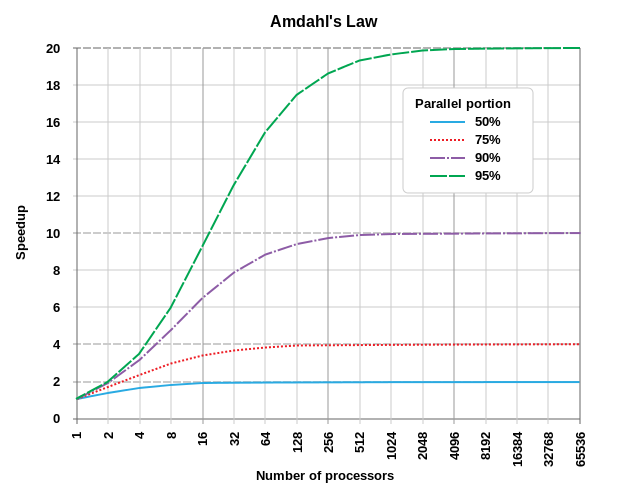
\includegraphics[width=0.65\textwidth]{AmdahlsLaw}
    \caption{Evolution of speedup with available processors}
    \label{fig:AmdahlsLaw}
\end{figure}
Figure(\ref{fig:AmdahlsLaw}) shows a non-linear scaling of speedup with addition of every new processor and 
further addition causes no performance improvement.\\

{\bfseries Consequences of the law:} 
\begin{itemize}
    \item small portions of sequential work impacts scalability
    \item in most practical (non-ideal cases), perfect scaling within a parallel code is hard due to
        \begin{itemize}
            \item Communication and Synchronization
            \item Resource bottlenecks (Memory bandwidth, Hyperthreading, etc.)
        \end{itemize}
    \item Load imbalance
\end{itemize}

\section{Common methodologies for parallelism}
{\bfseries A) Multiple Concurrent Execution or SPMD:}
\begin{itemize}
    \item Multiple Concurrent Executions (CEs)
    \item Distributed data
    \item Communication between Parallel Executions (PEs)
\end{itemize}

Advantages: limited orchestration overhead, explicit mapping of problems\\
Disadvantages: need to explicitly split data, possibility of load imbalance\\

{\bfseries B) Master/Worker:}\\ 
Central work queue at the master and workers ask for tasks from the master.

Advantages: simple approach, easy load balancing\\
Disadvantages: extra orchestration overhead, memory requirements (at masters), more communication, scalability 
challenges\\

{\bfseries C) Pipelining:}
\begin{itemize}
    \item Split functionality among PEs
    \item Pass "task" once functionility is done
\end{itemize}

Advantages: specialized units of task in parallel execution\\
Disadvantages: more communication and limited parallelism\\

{\small\fbox{
    \parbox[h]{\textwidth}{
        {\bfseries Data Parallelism v/s Functional Parallelism}

        \begin{enumerate}[label=(\bfseries \alph*)]
            \item {\bfseries Data Parallelism (e.g., SPMD):} 
                    \begin{itemize}
                        \item Same operations executed parallely for elements of a large data, say, arrays
                        \item Tasks are the operations on each individual elements or on subsets of the elements
                        \item Length of the task whether same or different depends on the application
                    \end{itemize}

            \item {\bfseries Functional Parallelism (e.g. Pipelining):} 
                    \begin{itemize}
                        \item Entirely different calculations can be performed concurrently on either the same or 
                                different data
                        \item Tasks are usually specified via different functions or code regions
                        \item The degree of available functional parallelism is usually modest
                        \item Tasks are of different length in most cases
                    \end{itemize}
            
        \end{enumerate}
    }
}}

\section{Flynn's Taxonomy/Classification}
\begin{enumerate}[label=(\bfseries \alph*)]
    \item {\bfseries SISD:} Single Instruction, Single Data (Sequential Processing)
    \item {\bfseries SIMD:} Single Instruction, Multiple Data (Pipelines, Vectors, GPUs); \\ \hspace*{1.15cm} Synchronized 
                            execution of the same instruction on a set of data; \\ \hspace*{1.15cm} Vector Programming like
                            CUDA, OpenGL, and so on
    \item {\bfseries MISD:} Multiple Instruction, Single Data (???/Systolic Arrays). 
    \item {\bfseries MIMD:} Multiple Instruction, Multiple Data (MPP Systems Clusters). \\ \hspace*{1.3cm} Asynchronous 
            execution of different instructions
\end{enumerate}

SIMD and MISD are the relevant items covering parallel systems and shall be focused on hereon.\footnote[8]{An important thing to
note here is the difference between a core and a processor. {\bfseries Processor} is the entire chipset including all the 
cores. {\bfseries Cores} are like 2 (or more like 4 core, 6 core) parts of the processor that does parallel processing 
(processing two different data simultaneously in different units) without causing much strain on the processor.} 

Classification of Parallel System can be seen in the figure below:
\begin{figure}[h]
    \centering
    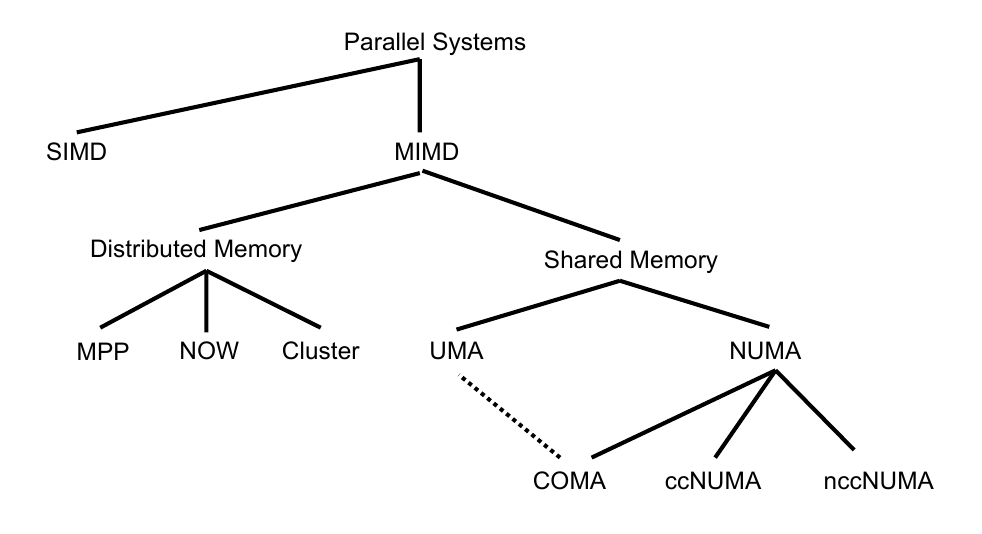
\includegraphics[width=0.60\textwidth]{Parallel_Systems}
    \caption{Classification tree for Parallel Systems}
    \label{fig:ParallelSystems}
\end{figure}

{\small\fbox{
    \parbox[h]{\textwidth}{
        {\bfseries Overview on SIMD and MIMD:}

        \begin{itemize}
            \item {\bfseries SIMD} is based on vector programming in form of pragmas (many vectorizing compilers)
                    \begin{itemize}
                        \item one instruction operates on a many data streams
                        \item GPGPU (General Purpose Computing on Graphics Processing Units) fits this model
                    \end{itemize}
        \end{itemize}

        \begin{center}
            {\bfseries whereas}
        \end{center}
        \begin{itemize}
            \item {\bfseries MIMD} has two different programming models:
                    \begin{enumerate}[label=\bfseries (\alph*)]
                        \item {\bfseries Shared Memory (SM) Programming}  matching shared memory architecture
                            \begin{itemize}
                                \item Multiprocessor System
                                \item System provides a shared address space
                                \item Communication is based on read/write operation to global addresses
                            \end{itemize}

                        \item {\bfseries Distributed Memory (DM) Programming}  matching distributed memory architecture
                            \begin{itemize}
                                \item Multicomputer System
                                \item Building blocks are nodes with private physical space
                                \item Communication is based on messages
                            \end{itemize}
                    \end{enumerate}
        \end{itemize}
    }
}}

\subsection{Shared Memory}
The Shared Memory Systems have the following architectures:
\begin{enumerate}[label=\bfseries (\Alph*)]
    \item {\bfseries Uniform Memory Access (UMA):} Symmetric Multiprocessors SMP architecture
            \begin{itemize}
                \item Centralized shared memory
                \item Access to global memory from all processors have "same latency"
                \item Transition from bus to crossbars
                \item Memory contention high\footnote[4]{{\bfseries Memory or CPU contention:} It is an event wherein 
                        individual CPU components and machines in a virtualized hardware system wait too long for their 
                        turn at processing.\\[-0.7em]}: as more CPUs are added, competition for access to the bus leads 
                        to a decline in performance.
            \end{itemize} 

    \item {\bfseries Non-uniform Memory Access (NUMA):} Distributed Shared Memory Systems - HW-DSM\footnote[1]{{\bfseries HW-DSM:} Hardware DSM\\[-0.7em]}
            \begin{itemize}
                \item Memory Distributed among the nodes
                \item Local accesses much faster than the remote ones
                \item Memory contention low: A processor's own internal computation can be done in its local memory, causing
                        a reduction in memory contention
            \end{itemize}

    \item {\bfseries More exotic:}
            \begin{itemize}
                \item {\bfseries COMA (Cache only):} Cache\footnote[2]{A {\bfseries CPU cache} (or simply {\bfseries cache}) is a 
                        hardware cache used by the central processing unit (CPU) of a computer to reduce the average cost (time or 
                        energy) to access data from the main memory. A cache is a smaller, faster memory, closer to a processor core,
                        which stores copies of the data from frequently used main memory locations.\\[-0.7em]} only memory architecture 
                        (COMA) is a computer memory organization for use in multiprocessors in which the local memories (typically DRAM) at 
                        each node are used as cache. This is in contrast to using the local memories as actual main memory, as in
                        NUMA organizations.
                \item {\bfseries ncc-COMA (Non-cache coherent)}\footnote[3]{{\bfseries Cache coherence:} A cache can be used
                        to improve the performance of accessing a given resource. When there are several such caches for the
                        same resource, as shown in the picture, this can lead to problems. {\bfseries Cache coherence} or 
                        {\bfseries Cache coherency} refers to a number of ways to make sure all the caches of the resource 
                        have the same data, and that the data in the caches makes sense (called data integrity). Cache coherence
                        is a special case of memory coherence.}  
            \end{itemize}
\end{enumerate}

\subsection{Shared Memory Models match Shared Memory}
Mechanism features of shared memory with the details are as follows:
\begin{enumerate}[label={\bfseries (\Alph*)}]
    \item {\bfseries Assumes a global address space with random access}
        \begin{itemize}
            \item any read/write can reach any memory cell 
            \item this is true for NUMA as well except that locality becomes tricky
            \item most models assume cache coherency
        \end{itemize}

    \item {\bfseries Communication through memory access}
        \begin{itemize}
            \item load/store operations to arbitrary address
            \item pass data from PE to the next
        \end{itemize}
    
    \item {\bfseries Synchronization constructs to coordinate accesses}
        \begin{itemize}
            \item need to ensure consistency, i.e., data synchronization
            \item need to ensure control flow, i.e., control synchronization 
        \end{itemize}
\end{enumerate}

{\bfseries Examples:} POSIX threads, OpenMP, \ldots

\section{Distributed Memory}
\subsection{Distributed Memory Models match Distributed Memory}
Mechanism features of distributed memory with the details are as follows:
\begin{enumerate}[label={\bfseries (\Alph*)}]
    \item {\bfseries Assumes no global address space}
        \begin{itemize}
            \item independent nodes with their own memory connected via network
            \item no direct visibility of data
        \end{itemize}
    
    \item {\bfseries All the communications via messages}
        \begin{itemize}
            \item Explicit Send/Recv pairs
            \item Remote memory access via get/put is also an option
            \item Messages carry data and synchronization
        \end{itemize}
\end{enumerate}

{\bfseries Examples:} MPI, PVM

\section{Hybrid Programming}
Most programming structures are hybrid due to their versatility.

\subsection{Rationale for Hybrid Programming to appear in programming models:}
\begin{itemize}
    \item pure shared memory models do not scale beyond node: memory contention
    \item pure message passing models create on-node performance issues
            \begin{itemize}
                \item longer latency than necessary
                \item too many message endpoints
            \end{itemize}
\end{itemize}

\subsection{Mapping: Critical Step in Hybrid Programming implementation}
\begin{enumerate}[label=\bfseries (\alph*)]
    \item {\bfseries Which task to execute where?}
        \begin{itemize}
            \item What to express in shared memory and what in message passing?
            \item What to map to threads and processes?
            \item Where to locate processes and threads (statically or dynamically)?
        \end{itemize}

    \item {\bfseries Some key issues to consider}
        \begin{itemize}
            \item Increase data locality
            \item Minimizing communications
            \item Resource contention (similar to memory contention)
            \item Memory usage
        \end{itemize}
\end{enumerate}
%=====================================================================================================================






%=====================================================================================================================
\chapter{Threading}
\begin{tcolorbox}[width=\textwidth,colback={white},title={In this chapter\dots},colbacktitle={lightslategray},coltitle=white]    
    \begin{itemize}
        \item Threading concepts
        \item Threading APIs
        \item POSIX Threads
    \end{itemize}
 \end{tcolorbox}
 
\section{Threads - Basics}
A {\bfseries{Thread}} of execution is the smallest sequence of programmed instructions that can be managed independently 
by a scheduler, which is typically a part of the operating system. 

\begin{itemize}
    \item A thread is a component of the process.
    \item Multiple thread can exist within a process {\bfseries executing} concurrently and {\bfseries sharing} the 
          resources like memory, while different process do not share these resources.
\end{itemize}

\begin{figure}[h]
    \centering
    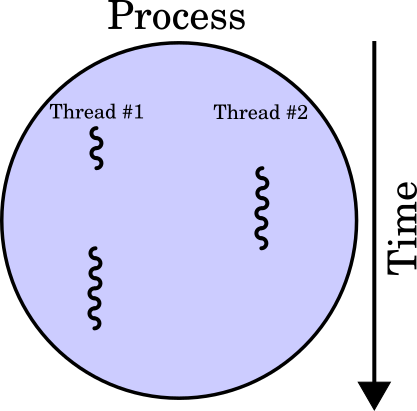
\includegraphics[width=0.20\textwidth]{Multithreadedprocess}
    \caption{Diagramatic representation of Processes and corresponding threads}
    \label{fig:Threads}
\end{figure}

{\large{\bfseries{Hardware threads and Software threads}}}\\
{\bfseries{Hardware Threads:}}
It is the execution of the execution stream inside the hardware (similar von Neumann machine in hardware). A Separate 
Control Unit executing a sequence of instructions.\\

{\bfseries{Software Threads:}}
These are programming abstractions that represent a stream of execution and remain exposed to programmer.

{\textit {To execute a program.}} This happens with the software and harware coming together. \\
A programmer defines a software thread which then gets mapped to hardware thread for execution.


\subsection{Hyperthreading/SMT - Simultaneous multithreading}
{\bfseries{Hyperthreading}} is intel's proprietary simultaneous multithreading to improve the parallelization of
computation.
For each physical core on the processor, the Operating system addresses to virtual(logical) cores and shares work load
between them when possible. Hyperthreads also show up as "CPUs" and not distingushable by default. BIOS initializes them
along with cores and sockets as boot which require a reboot for changes. 

{\textit{Functions and Salient Features}}:
\begin{itemize}
    \item The main function of hyper-threading is to increase the number of independent instructions in the pipeline
    \item It takes advantage of the superscalar architecture, in which multiple instructions work on separate data in
          parallel
    \item Concurrent workloads: With HTT, one physical processor core appears as two to the operating system, allowing 
          concurrent scheduling of two processes per core
    \item Resource Sharing: In addition two two or more processes can use the same resources: if resources of one 
          process are not available, then another process can continue if its resources are available
    \item Mostly useful for systems daemons and I/O operations
\end{itemize}

{\textit{Problems with Hyperthreading use in parallel programming}}. 
\begin{itemize}
    \item multiple instances of same program with same resource requirements
    \item the above often causing heavy impacts on speedup 
    \item a careful need to understand what needs to be scheduled on HT/SMT 
\end{itemize}

\subsection{Software Threading Basics}
\begin{itemize}
    \item Traditional view:
        \begin{itemize}
            \item Operating systems maintain processes which get scheduled to available hardware threads (aka. processors).
                  Each process has one execution stream.\\
                  ({\bfseries{Stream processing}} is about processing continuous streams of data by programs in a workflow.\\ 
                  {\bfseries {Continuous execution}} is discretized by grouping input stream tuples into batches and 
                  using one batch at a time for the execution of programs.)
        \end{itemize}
    \item Processes maintain isolation for protection by separating address space and files. They are:
        \begin{itemize}
            \item coupled with user IDs 
            \item communication only via IPC (Inter-Process Communication)
        \end{itemize}
    \item Threading was intended to make things easier by:
        \begin{itemize}
            \item Sharing of data without protection boundaries with cooperative behavior to support asynchronous 
                  behaviour\\
                  ({\bfseries{Synchronous}}, or {\bfseries{Synchronized}} means "connected", or "dependent" in some way.
                  In other words, two synchronous tasks must be aware of one another, and one task must execute in some 
                  way that is dependent on the other, such as wait to start until the other task has completed.\\
                  {\bfseries Asynchronous} means they are totally independent and neither one must consider the other in
                  any way, either in initiation or in execution.)
            \item OS still responsible for rescheduling (preemption and progress)
        \end{itemize}
\end{itemize}

\subsection{User-Level Threads}
{\bfseries{User-Level threads}}, unlike Hyperthreads that require kernel-level modifications, are managed entirely by the
run-time system (user-level library).\\
{\textit{Features :}}
\begin{itemize}
    \item The kernel knows nothing about user-level threads and manages them as if they were single-threaded processes
    \item User-level threads are small and fast, each thread is represented by a PC, register, stack, and small thread
          control block
    \item Switch between threads is easy and can be done as needed
    \item Use cases:
            \begin{itemize}
                \item Light weight, fine-grained task based parallel programming 
                \item Closely coordinated activities with well-defined switchpoints
            \end{itemize}
\end{itemize}

{\textit{Disadvantages.}} There is no guarantee for scheduling as preemption and progress is very hard to guarantee (if 
not impossible).\\

{\large{\bfseries{Process and its components:}}}\\
A {\bfseries process} is an instance of a program that is being executed by one or many threads. It contains the program
code and its activity. Depending on the operating system, a process may have multiple threads of execution that execute 
instructions concurrently.

{\textit{Component of a process}}. A process in general is said to own the following resources:
\begin{itemize}
    \item an {\bfseries image} of the executable machine code associated with a program
    \item {\bfseries{Memory}} that include the following:
            \begin{itemize}
                \item executable code
                \item process-specific data (input and output)
                \item a {\bfseries{call stack}} to keep track of active subroutines and/or other events
                \item a {\bfseries{heap}} to hold intermediate computation data generated during runtime
            \end{itemize}
    \item Operating system {\bfseries{descriptors}} of resources allocated to the process for the execution of the instruction
          such as file descriptors (UNIX terminology) or handles (Windows)
    \item Security attributes, such as process owners and the process' set of permissions (permissible operations)
    \item {\bfseries{Processor state}} such as the content of registers and physical memory addressing
\end{itemize}

{\large{NOTE.}} Though a process has all the components similar to an OS, it doesn't execute on its own.

\subsection{Rationale for Threads in Parallel Programming}
The {\bfseries{traditional use}} of threads is {\bfseries{concurrency}}, however, they can as well be used for parallel 
programming. Threads expose hardware threads to programmer and {\bfseries{acts as a native interface to access parallelism}} in 
the architecture.

Thus, the following motivations to talk about threads in Parallel Programming:
\begin{itemize}
    \item Motivation 1:
            \begin{itemize}
                \item exploit hardware threads as directly as possible
                \item direct mapping to resources
                \item understanding bottlenecks and overheads where they occur
            \end{itemize}
    \item Motivation 2:
            \begin{itemize}
                \item runtime systems for parallel programming build on them, example, OpenMP
                \item properties of threads and how their usage have a large impact on performance
            \end{itemize}
\end{itemize}


{\textit{Programming with Threads.}} Threads are mostly programmed as packages that are {\bfseries{mapped to native APIs}} (like
POSIX threads, Win32 threads, Solaris threads, and Java threads) and are often {\bfseries{user-level threads}}.\\

{\textit{Motivation for custom APIs}}. Lower overheads, customized for particular tasks, and custom hardware with special
properties.

\section{POSIX Threading}
\subsection{Fork/Join Model}
In parallel computing, the {\bfseries{fork-join model}} is a way of setting up and executing parallel programs, such that execution
"branches-off" (fork) in parallel at designated points in the program, to "merges" (join) at a subsequent point and resume
sequential execution.\\
All the threads operate concurrently and location is transparent at first. At the end of the parallel regions, master waits for other
thread to complete and continues the sequential execution. 

{\bfseries{Syntax}}:
\begin{itemize}
    \item {\bfseries{Header:}} \begin{verbatim} #include <pthread.h> \end{verbatim}
    \item {\bfseries{Keyword identifier:}} \begin{verbatim} pthread_t \end{verbatim}
    \item {\bfseries{Creating a thread (Fork):}}   
    \begin{verbatim} 
        int pthread_create( pthread_t *thread,
                            const pthread_attr_t *attr,
                            (void*) *kernel (void*),
                            void* args );
    \end{verbatim}
    \item {\bfseries{Termination of parallel threads (Join):}}
    \begin{verbatim}
        int pthread_join(   pthread_t thread,
                            void* (*retval) );
    \end{verbatim}
\end{itemize}

\section{Synchronization between threads}
Unless pure concurrency, i.e., independent tasks and no dependencies on allocation computing resources, the threads need to be 
synchronized.\\
Common examples to show the need for synchronization are: enforcing common completion of task, enforce happens before initiation 
into the parallel regions and guard updates to common control unit assigned to the process. \\
{\bfseries{Two main concepts of Synchronization in POSIX threads.}} 
\begin{itemize}
    \item Locks/Mutual Exclusion (mutex), 
    \item Condition Variables
\end{itemize}

\subsection*{Concept A: Mutual Exclusion}
Mutual Exclusion, also called {\bfseries{mutex}}, is used for problems of {\bfseries{concurrent access to shared resources}}.These
can be:
\begin{itemize}
    \item shared variables, memory locations
    \item access to I/O
    \item two or more threads concurrently updating a variable leading to inconsistencies
\end{itemize}

{\bfseries{API Syntax}}:
\begin{itemize}
    \item {\bfseries{Variable Identifier/keyword:}} \begin{verbatim} pthread_mutex_t \end{verbatim} 
    \item {\bfseries{Initialization:}}  \begin{verbatim} PTHREAD_MUTEX_INITIALIZER \end{verbatim}
          and written as \begin{verbatim} pthread_mutex_t mutexname = PTHREAD_MUTEX_INITIALIZER; \end{verbatim}
          or dynamically as: 
        \begin{verbatim} 
            int pthread_mutex_init( pthread_mutex_t &mutexname,
                                    const pthread_mutexattr_t *attr ); 
            int pthread_mutex_destroy( pthread_mutex_t &mutexname ); 
        \end{verbatim}
        Here, for mutex attributes one can do: \begin{verbatim} pthread_mutexattr_t *attr = PTHREAD_MUTEX_RECURSIVE; \end{verbatim}
    \item {\bfseries{Lock a mutex:}} blocks until mutex is granted
          \begin{verbatim} int pthread_mutex_lock( &mutexname ); \end{verbatim}
    \item {\bfseries{Unlock a mutex:}} returns immediately
          \begin{verbatim} int pthread_mutex_unlock( &mutexname ); \end{verbatim}
    \item {\bfseries{Lock a mutex, if available:}} returns immediately
          \begin{verbatim} int pthread_mutex_trylock( &mutexname ); \end{verbatim}
\end{itemize}

{\texttt {mutex}} is a standalone variable that is not explicitly associated with the memory it protects. It is thus the programmmer's
responsibility for its correct usage.\\
{\textit{Critierion for implementations of locks.}} Correctness: gaurantees mutual exclusion, every process gets the mutex, fairness.

\subsection*{Concept B: \texttt{<atomic>} Operations}
In general from a C++ standpoint, \texttt{<atomic>} types are types that encapsulate a value whose access is gauranteed to not cause 
data races{\footnote[2]{A {\bfseries{race condition}} is an undesirable situation that occurs when a device or system attempts to 
perform two or more operations at the same time, but because of the nature of the device or system, the operation must be done in a 
proper sequence to be done correctly. This leads to an inconsistent output}} and can be used to synchronize the memory access to shared 
resources from different concurrent threads. \\
Common examples in threading are: test and set; compare and swap
\begin{verbatim}
    volatile int *mutex;
    void lock()
    { while(test_and_set(&mutex) == 1); }
\end{verbatim}

\subsection*{Concept C: Condition Variables}
This is another way of prevention of undesirable behaviour as a result when two or more threads try to access and/or manipulation the 
input at a given memory location. The key features of condition variables are:
\begin{itemize}
    \item Waiting is based on the shared variable value and it works in conjugation with a mutex variable to protect that data
    \item A thread needs to wait till a condition is true and therefore, blocked until this happens
    \item A different threads keeps checking the conditions and once met signals the other threads about this
\end{itemize}

{\bfseries{API Syntax:}}
\begin{itemize}
\item {\bfseries{Variable Identifier/keyword:}} \begin{verbatim} pthread_cond_t \end{verbatim} 
\item {\bfseries{Initialization:}}  \begin{verbatim} PTHREAD_COND_INITIALIZER \end{verbatim}
      and written as \begin{verbatim} pthread_cond_t condition_variable = PTHREAD_COND_INITIALIZER; \end{verbatim}
      or dynamically as: 
    \begin{verbatim} 
        int pthread_cond_init(      pthread_cond_t &condition_variable,
                                    const pthread_cond_attr *attr );
        int pthread_cond_destroy(   pthread_cond_t &condition_variable );
    \end{verbatim}
\item {\bfseries{Wait on a condition to be set in another thread:}} 
        \begin{itemize}
            \item unlocks mutex, blocks until conditions is signaled, acquires lock
            \item Mutex must be locked before calling
    \begin{verbatim}
        int pthread_cond_wait(  &condition_variable,
                                &mutex );
    \end{verbatim}
        \end{itemize}
\item {\bfseries{Signal a condition to a waiting thread:}} 
        \begin{itemize}
            \item send condition to other thread
            \item must be followed by an unlock
    \begin{verbatim}
        int pthread_cond_signal(    &mutex );
        int pthread_cond_broadcast( &mutex );
    \end{verbatim}
        \end{itemize}
\end{itemize}

\subsection*{Concepts D: Miscellaneous}
{\bfseries{Barriers}}\\
It is a point in the program where we want all the threads to reach before continuing with further executions. This is a very useful 
tool for synchronization.\\
{\bfseries{API Syntax}}:
\begin{itemize}
    \item {\bfseries{Variable Identifier/keyword:}} \begin{verbatim} pthread_barrier_t \end{verbatim} 
    \item {\bfseries{Initialization:}} Done dynamically as: 
    \begin{verbatim} 
        int pthread_barrier_init(       pthread_barrier_t *barrier,
                                        const pthread_barrierattr_t *attr,
                                        unsigned int count ) 
        int pthread_barrier_destroy(    pthread_barrier_t *barrier ) 
    \end{verbatim}
    \item {\bfseries{Wait for the threads to complete their processing:}}
          \begin{verbatim} int pthread_barrier_wait( *barrier ) \end{verbatim}
\end{itemize}


\subsection{Performance Aspects for Threading}
The primary aspects that impact the perfomance of the threads are:
\begin{itemize}
    \item {\bfseries {Overheads}}: thread creation and destruction can be a very expensive process, so ensure that the parallel regions 
          are large        
    \item {\bfseries{Contention:}}
        \begin{itemize}
            \item Locks are low-overhead when few threads try access them
            \item These overheads grow with more threads accessing them more often indicating high resource contention
        \end{itemize}
    \item {\bfseries{Thread pinning}}: also called {\bfseries{cache affinity/processor affinity}}, enables the binding and unbinding of 
          a process or a thread to a CPU or a range of CPUs, so that the process or thread will execute only on the designated CPU(s) 
          rather than any CPU.\\
          Advantage of this is that remnants of a process that was run on a processor may remain in that same processor's state after
          another process was run on it. This improves the performance by reducing the performance reducing performance-degrading events
          such as {\bfseries{cache misses}} \footnote[8]{A {\bfseries{cache miss}} is a state where the requested data for processing
          of a component of application is not found in the cache memory causing execution delay as the data has to be fetched from 
          other cache levels or main memory.} \\
          In the context of the given topic, for system-level threads the OS does scheduling of the SW thread to the HW thread, therefore,
          deciding the location of a thread's execution that largely impacts the performance. {\bfseries{Pinning or fixing}} a SW thread 
          to a hardware thread improves the performance due to the above stated reasons.\\
          {\bfseries{NOTE:} Thread pinning becomes extremely complicated on a NUMA architecture. Also, thread pinning does not solve 
          the persistent load-balancing problem.}
\end{itemize}


\subsection{Lock Granularity}
Lock Granularity deals with the cost of implementing locks depending upon the space and time where space refers to the data structure of 
the DBMS{\footnote[3]{{\bfseries{DBMS:}} Database Management System}} for each lock and time refers to the handling of the lock requests 
and release. The cost of lock implementation depends on the size of data items. There are two types of lock granularity:
\begin{itemize}
    \item {\bfseries{Fine Granularity:}} It refers to small item sizes
            \begin{itemize}
                \item one lock for each data element
                \item maximizes concurrency (multiple threads can have lock at a time)
                \item require multiple locks and many locking calls at the same time making the implementation complicated
            \end{itemize}
    \item {\bfseries{Coarse Granularity:}} It refers to large item sizes. 
            \begin{itemize}
                \item one single lock for all data
                \item limits concurrency
                \item easy to implement
            \end{itemize}
\end{itemize}
A too-fine lock granularity will increase the frequency for the lock requests and lock releases which will add additional instructions.\\
A too-coarse lock granularity increases the idle state of threads as they wait longer for acquiring the locks. Also, upon acquiring the 
lock, they would take longer to execute the larger data increasing the waiting time for other threads. This limits concurrency.

\section{Drawbacks of Pthreads}
\begin{itemize}
    \item {\bfseries {Pthreads represent direct abstraction of system-level parallelism}}
            \begin{itemize}
                \item Direct map to underlying hardware threads (in most cases)
                \item Even parallel loops are difficult to think about
            \end{itemize}
    \item {\bfseries{Association of data and threads is up to the programmer}}
            \begin{itemize}
                \item No program construct to do this
                \item Data locality has to be done explicitly
            \end{itemize}
    \item {\bfseries {Need to manage the data visibility manually}} such as variables per thread and variables shared across the threads
    \item {\bfseries{Simple synchronization primitives}}; these are not sufficient to do easy parallel coordination
\end{itemize}
%=====================================================================================================================





%=====================================================================================================================
\chapter{OpenMP - Open Multi-Processing and Shared Memory Systems}
\begin{tcolorbox}[width=\textwidth,colback={white},title={In this chapter\dots},colbacktitle={lightslategray},coltitle=white]    
    \begin{itemize}
        \item OpenMP Introductions
        \item Contructs of Worksharing within OpenMP
        \item Compiler Directive and Internal Control Variables (ICVs)
        \item Explicit Tasking and performance considerations
        \item Memory models in shared memory systems
        \item Dependence Analysis and Loop Transformations
        \item Challenges in Shared Memory Parallelism
    \end{itemize}
 \end{tcolorbox}

 \section{What is OpenMP? {\small{and what it is not?}}}
 OpenMP is an Application Program Interface (API) which is used to program multi-threaded, shared memory parallelism (plus accelerators)
 usually of the type UMA and NUMA.\\
 {\textit{Primary component of OpenMP API.}} They are:
 \begin{itemize}
     \item {\bfseries{Compiler Directives (for C/C++ and Fortran)}}
     \item {\bfseries{Runtime Library Routines}}
     \item {\bfseries{Environment Variables}}
 \end{itemize}

 {\textit{What it is not intended to be?}}\\
 OpenMP is {\bfseries{NOT}} \dots 
 \begin{itemize}
     \item intended for distributed memory systems
     \item necessarily implemented identically by all vendors
     \item guaranteed to automatically make the most efficient use of shared memory
     \item required to check for data dependencies, race condition, deadlocks, etc.
     \item designed to handle parallel I/O
 \end{itemize}

{\bfseries{API Syntax:}}
\begin{itemize}
    \item A simple example demonstrating the header for OpenMP and the use of the comiler directives for creating a parallel region
    \begin{verbatim}
        #include <omp.h>
        int main(){
            #pragma omp parallel        //Compiler Directive
            {
                printf("Hello World!\n");
            }
        }
    \end{verbatim}
    \item for compiling: {\texttt{gcc -O3 -openmp program.c}}
\end{itemize}

\subsection{Fork/Join Execution Model}
Similar to the model discussed in the Pthreads sections, the fork/join model goes as:
\begin{itemize}
    \item The execution of an openmp code begins with a single thread called {\bfseries{master thread}}
    \item Upon encountering the parallel region, the master threads creates additional threads
    \item After completion of the parallel region, the additional threads return to runtime
    \item The master thread then continues the execution sequentially
    \item Additionally, the parallel threads are synchronized at the end of every parallel region via an {\bfseries{(implicit) barrier}}
\end{itemize}

Also, the threads in the parallel region can themselves create additional thread all of which follow the same execution model as above.
Therefore, OpenMP is not required to spawn/use additional threads in the parallel region. 

\section{OpenMP Implementations}
While OpenMP implementations may differ from system to system, the following features remain inherent to all of them:
\begin{itemize}
    \item OpenMP is a {\bfseries{language extension}} usually over C/Fortran 
            \begin{itemize}
                \item Pragmas to the base language can be ignored during the usage
            \end{itemize}
    \item Due to the above, it {\bfseries{requires a new compiler}} which is built inside the existing one
    \item Additionally, OpenMP {\bfseries{requires runtime library}} which schedule the execution to the hardware threads. These libraries
          are often built over pthreads\\
          Standard defines some user functions but not the entire environment. Most common examples are Intel's OpenMP/LLVM, and so on
\end{itemize}
{\bfseries{NOTE:}} Well defined environment variables are also called {\bfseries{"Internal Control Variables" (ICVs)}}. Degree of parallelism
is controlled by ICV: $\quad$ {\texttt{OMP\textunderscore NUM\textunderscore THREADS}}

\subsection{OpenMP System Stack}
\begin{enumerate}[label={\bfseries{\alph*)}}]
    \item OpenMP Application
    \item Compiler Directives $\rightarrow$ OpenMP Runtime APIs $\rightarrow$ Environment Variables (ICVs)
    \item OpenMP Runtime Library
    \item Operating System (typically with system level threads, mostly POSIX threads)
    \item Memory Architecture (UMA or NUMA)
\end{enumerate}

\section{More on API Syntaxes and Compiler Directives}
\subsection{Sections in a Parallel Region}
This should appear within a parallel section. Each section inside the sections block is executed once by one of the threads. When a thread
finishes its section it waits for others threads at the ends of the sections block or region.

{\bfseries{API Syntaxes:}}
\begin{itemize}
    \item {\bfseries{General Syntax:}}
    \begin{verbatim}
        #pragma omp sections [parameters]
        {
            #pragma omp section
                //...task to be executed in the first section
            #pragma omp section
                //...task to be excecuted in the second section and so on.....
        }
    \end{verbatim}
    \item {\bfseries{Example:}}
    \begin{verbatim}
        int main(){
            int a[100], b[100];
            #pragma omp parallel                  
            {                           
                #pragma omp sections    //"Sections" block line
                {
                    #pragma omp section
                    for(int n = 0; n < 100; n++)
                        a[n] = 100;

                    #pragma omp section
                    for(int n = 0; n < 100; n++)
                        b[n] = 200;
                }
            }
        }
    \end{verbatim}
    To avoid writing the {\texttt{"Sections" block line}}, we can write the above code as:
    \begin{verbatim}
        int main(){
            int a[100], b[100];
            #pragma omp parallel sections                
            {                           
                #pragma omp section
                for(int n = 0; n < 100; n++)
                    a[n] = 100;

                #pragma omp section
                for(int n = 0; n < 100; n++)
                    b[n] = 200;
            }
        }
    \end{verbatim}
\end{itemize}

\subsection{Work Sharing in Parallel Region}
The important thing in the parallelism of shared memory, as in this case, is an easy construct for division of data in the parallel region.
Most important construct being that of loops escpecially {\texttt{for}} loops.

\subsubsection{Parallel Loop}
\begin{itemize}
    \item The iterations of the loop are distributed among the parallel threads that concurrently execute the loop
    \item There is no synchronization at the beginning of the loop
    \item However, each thread wait at the end of the loop by an implicit barrier for synchronization of the team of threads unless there is
          used of {\textit{nowait}}
    \item Note: the expressions in the for-statement are very restricted (constrained) in order to apply parallel for without inconsistent
          output
\end{itemize}

The constraints on the loop in order to obtain a consistent behavior while using this construct are:
\begin{itemize}
    \item no data dependencies
    \item can be implemented in any order
    \item since there is no programming construct available within OpenMP to do this, it is the responsibility of programmer to ensure this
\end{itemize}

{\bfseries{API Syntax(es)}}
\begin{itemize}
    \item {\bfseries{Compiler Directive:}} The compiler directive shown below must be followed by a {\texttt{for}} loop:
    \begin{verbatim}
        #pragma omp for
        for .....
    \end{verbatim}
    \item {\bfseries{Examples:}}
    \begin{verbatim}
        int main(){
            int a[100];
            #pragma omp parallel
            {
                #pragma omp for     //compiler directive line for "for"
                for(int n = 0; n < 100; n++)
                    a[n] =  1000;
            }
        }
    \end{verbatim}
    Alternatively, the {\texttt{compiler directive line for "for"}} can be done alternatively written with the compiler directive for 
    {\texttt{\textbf{parallel}}} region as shown below:
    \begin{verbatim}
        int main(){
            int a[100];
            #pragma omp parallel for
            {
                for(int n = 0; n < 100; n++)
                    a[n] = 1000;
            }
        }
    \end{verbatim}
\end{itemize}

\subsubsection*{How do Loops get split up?}
Iterations for a loop must be split between threads. Loop scheduling defines chunk size and decides how these are to be distributed amongst
the threads (or mapped to the threads). OpenMP provides several options under the construct {\texttt{schedule}}. The compiler directive is:\\
\verb$#pragma omp for schedule(<option name>, <chunk-size>)$

\subsubsection*{Available Loop Schedules}
\begin{itemize}
    \item {\texttt{static}}
    \begin{itemize}
        \item static scheduling with fixed size chunk (decided by the ratio of the iterations and the number of threads) distributed in a
              round robin fashion
        \item default size of {\texttt{chunk-size}} is 1
        \item threads are allocated the chunks in a sequential fashion, namely, first allocation to thread 1, then thread 2, and so on \dots
        \item this is used when all the iterations have the same computational cost
    \end{itemize}
    \item {\texttt{dynamic}}
    \begin{itemize}
        \item each threads executes a chunk of the specified size and then requests another chunk until no more chunks are left, hence, 
              dynamic allocation of chunks
        \item no particular order of allocation of chunk and it changes each time we execute the loop
        \item default size of {\texttt{chunk-size}} is 1
        \item {\texttt{dynamic}} scheduling is good when there is different computational cost associated with the iterations which mean that
              the iterations are poorly balanced between each other
        \item due to the dynamic scheduling it has a higher overhead in comparison to {\texttt{static}} scheduling
    \end{itemize}
    \item {\texttt{guided}}
    \begin{itemize}
        \item similar to {\texttt{dynamic}} scheduling: each thread executes a chunk of iterations and then requests another chunk
        \item the {\bfseries{difference}} is that at any instant the {\bfseries{size of chunk is proportional to the number of iterations left
              divided by the number of threads}}
        \item {\texttt{chunk-size}} decides the {\bfseries{minimum size of a chunk}}. However, the chunk which contains the last iterations
              may have size smaller than {\texttt{chunk-size}}
    \end{itemize}
    \item {\texttt{runtime}}
    \begin{itemize}
        \item the decision for scheduling in this case is deferred until the runtime
        \item there are different ways of specifying the scheduling type; one option is through the environment variable 
              {\texttt{OMP\textunderscore SCHEDULE}} and the other option is with the function 
              {\texttt{omp\textunderscore set\textunderscore schedule}}
    \end{itemize} 
    \item {\texttt{auto}}
    \begin{itemize}
        \item this scheduling delegates the decision of scheduling to the compiler and/or runtime system
    \end{itemize}
\end{itemize}

{\bfseries{Example for Loop Scheduling:}}
\begin{verbatim}
    #define S 25
    int main(int argc, char** argv){ 
        int a[S],b[S],c[S];
        #pragma omp parallel
        {
            #pragma omp for schedule(static)
            for (int i=0; i<S;i++)
                a[i] = omp_get_thread_num();
            #pragma omp for schedule(dynamic, 4)
            for (int i=0; i<S;i++)
                b[i] = omp_get_thread_num();
            #pragma omp for schedule(guided)
            for (int i=0; i<S;i++)
                c[i] = omp_get_thread_num();
        }
        for (int i=0; i<S;i++)
            printf(“Iter %4d: %4d %4d %4d\n",i,a[i],b[i],c[i]);
    }
\end{verbatim}
\begin{figure}[h]
    \centering
    \includegraphics[width=0.25\textwidth]{Scheduling}
    \caption{Output for the above program}
    \label{fig:Scheduling}
\end{figure}

\subsection{Data Visibility in Parallel}
In this part of chapter, we shall see how certain constructs affect the visibility of data across threads in a parallel region.

\subsubsection{Concept I: Shared v/s Private Data}
{\bfseries{Shared Data:}}
\begin{itemize}
    \item the clause {\texttt{shared(list)}} declares all the variables within {\texttt{list}} as shared
    \item this creates {\bfseries{one copy of the variables per thread}}
    \item {\bfseries{example}}: a reference {\texttt{a[5]}} to a shared array accesses
    \item OpenMP puts {\bfseries{no restriction to prevent data races between shared variables}}, thus making it the programmer's
          responsibility to assure prevention of such an event. This might cause to give an {\bfseries{inconsistent behavior after the parallel 
          region}} 
\end{itemize}

{\bfseries{Private Data:}}
\begin{itemize}
    \item with the clause \verb$private(list)$, OpenMP replicates the variables and assigns its local copy to each thread.
    \item {\bfseries{Each thread gets its own unique memory where it should store the value of the variable while in the parllel region}}.
          Therefore, the variable copy is accessible only by the thread that owns it. After the parallel region ends, the memory is freed and 
          these variable no longer exist
    \item private variables sometimes have an {\bfseries{unintuitive behavior in parallel region}}.\\
          {\bfseries{Following important remarks:}} Assume a private variable has value before the parallel region. However, {\bfseries{the value
          of the variable at the beginning of parallel region is undefined}}. Additionally, the value of the variable is the same as the 
          initialized value before the parallel region, in case of initialization. In case uninitialized, the value after the parallel region is
          inconsistent
    \item {\bfseries{NOTE:}} Iterator variables are {\bfseries{private by default}}
\end{itemize}

{\bfseries{Scope of certain variable:}}
\begin{itemize}
    \item the default for global variables: {\bfseries{shared}}
    \item variables defined within the "dynamic extent" of the parallel regions: {\bfseries{local}}. This also includes routines called from
          within the parallel regions
\end{itemize}

\subsubsection*{Some examples of the Private and Shared data:}
{\bfseries{Example A:}}
\begin{verbatim}
    int main(){
        int a[100], t, n;
        #pragma omp parallel
        {
            #pragma omp for private(t)
            for(int i = 1; i<n; i++){
                t    = f(i);
                a[i] = t;
            }
        }
    }
\end{verbatim}
{\bfseries{Global Variable}}: a, t, n\\
{\bfseries{Local varible to threads}}: i (by default since it is an {\bfseries{iterator variable}})\\
Variable {\texttt{t}} by default was shared but is now "privatized"\\
\\
{\bfseries{Example B:}}
\begin{verbatim}
    int main (){
        int iam, nthreads;
        #pragma omp parallel private(iam,nthreads)
        {
            iam = omp_get_thread_num();
            nthreads = omp_get_num_threads();
            printf(“ThradID %d, out of %d threads\n”, iam, nthreads);
            if (iam == 0)
            printf(“Here is the Master Thread.\n”);
            else
            printf(“Here is another thread.\n”);
        }
    }
\end{verbatim}
{\bfseries{REMARKS:}} A better programming practice is to declare {\texttt{iam, nthreads}} within the parallel region as these are being used
privately. Doing that alters the compiler directive to:\\ \verb$#pragma omp parallel$\\
\\
{\bfseries{Example C: Outputs in private and shared options}}
\begin{itemize}
    \item example for \verb$shared$ case
    \begin{verbatim}
        int i=3;
        #pragma omp parallel for
        for (int j=0; j<4; j++){
            i=i+1;
            printf("-> i=%d\n", i); 
        }
        printf("Final Value of I=%d\n", i);
    \end{verbatim}
    \begin{itemize}
        \item Output for {\bfseries{first run}}: \qquad\qquad\qquad\qquad\qquad\textendash\hspace{0.2em} Output for {\bfseries{second run}}:
        \begin{verbatim}
            -> i=4                                  -> i=4
            -> i=7                                  -> i=5
            -> i=6                                  -> i=4
            -> i=5                                  -> i=4
            Final Value of I=7                      Final Value of I=5
        \end{verbatim}
        \item Since OpenMP has no preventive contruct for data race, the value of the shared variable \verb$i$ is inconsistent after the parallel
              loop finsihes 
    \end{itemize}
    \item example for \verb$private$ case
    \begin{verbatim}
        int i=3;
        #pragma omp parallel for private(i)
        for (int j=0; j<4; j++){
            i=i+1;
            printf("-> i=%d\n", i); 
        }
        printf("Final Value of I=%d\n", i);
    \end{verbatim}
    \begin{itemize}
        \item Output for the above: 
        \begin{verbatim}
            -> i=?
            -> i=?
            -> i=?
            -> i=?
            Final Value of I=3
        \end{verbatim}
        \item the parallel region shows an undefined value for \verb$i$. However, at the end of the parallel region, the value resumes with
              the one used for initialization before the parallel region 
    \end{itemize}
\end{itemize}

\subsubsection{Concept II: First/Last Private Data}
This section is a following the concept of \verb$private$ data. Thus, we would consider that as the preceding idea as we move through this 
section.\\
\\
{\bfseries{Last Private:}}
\begin{itemize}
    \item Unlike, the \verb$private$ data beahavior, if we want the private data to take forward the last value of the parallel region, we would
          use \verb$lastprivate$
    \item {\bfseries{Example A:}}
    \begin{verbatim}
        int i=3;
        #pragma omp parallel for lastprivate(i)
        for (int j=0; j<4; j++){ 
            i=i+1;
            printf("-> i=%d\n", i); 
        }
        printf("Final Value of I=%d\n", i);
    \end{verbatim}
    \begin{itemize}
        \item Output for above is:
        \begin{verbatim}
            -> i=?
            -> i=?
            -> i=?
            -> i=?
            Final Value of I=?
        \end{verbatim}
        \item {\bfseries{Remarks:}} The output is undefined since the value of \verb$i$ is undefined at the beginning of the parallel region. 
              Let's see another example
    \end{itemize}
    \item {\bfseries{Example B:}}
    \begin{verbatim}
        int i;
        int x;
        x=44;
        #pragma omp parallel for lastprivate(x)
        for(i=0;i<=3;i++){
            x=i;
            printf("Thread number: %d     x: %d\n",omp_get_thread_num(),x);
        }
        printf("x is %d\n", x);
    \end{verbatim}
    \begin{itemize}
        \item Output for above is:
        \begin{verbatim}
            Thread number: 0     x: 0
            Thread number: 3     x: 3
            Thread number: 2     x: 2
            Thread number: 1     x: 1
            x is 3
        \end{verbatim}
        \item {\bfseries{Remarks:}} The output is \verb$3$ and not \verb$1$, i.e., {\bfseries{it is the last iteration and not the last operation}}
              that is kept
    \end{itemize}
\end{itemize}

{\bfseries{First Private:}}\\
To understand what happens with the use of the keyword \verb$firstprivate$, we make changes to the examples used for \verb$lastprivate$ section.
\begin{itemize}
    \item \verb$firstprivate$ specifies that each thread should have its own instance of a variable (like in case of \verb$private$) and that the
          variable {\bfseries{should be initialized to the value of the variable before the parallel construct}}
    \item {\bfseries{Example C:}}
    \begin{verbatim}
        int i=3;
        #pragma omp parallel for firstprivate(i)
        for (int j=0; j<4; j++){ 
            i=i+1;
            printf("-> i=%d\n", i); 
        }
        printf("Final Value of I=%d\n", i);
    \end{verbatim}
    \begin{itemize}
        \item Output for above is:
        \begin{verbatim}
            -> i=4
            -> i=4
            -> i=4
            -> i=4
            Final Value of I=3
        \end{verbatim}
    \end{itemize}
    \item {\bfseries{Example D:}}
    \begin{verbatim}
        int i;
        int x;
        x=44;
        #pragma omp parallel for firstprivate(x)
        for(i=0;i<=3;i++){
            x=i;
            printf("Thread number: %d     x: %d\n",omp_get_thread_num(),x);
        }
        printf("x is %d\n", x);
    \end{verbatim}
    \begin{itemize}
        \item Output for above is:
        \begin{verbatim}
            Thread number: 0     x: 0
            Thread number: 3     x: 3
            Thread number: 2     x: 2
            Thread number: 1     x: 1
            x is 44
        \end{verbatim}
    \end{itemize}
    \item {\bfseries{Remarks on both examples' outputs:}} As discussed above the outputs in the both case, i.e., \verb$x=44$ and \verb$I=3$
          are the values of the variable to which it was initialized before the parallel construct
\end{itemize}

{\bfseries{First Private and Last Private:}}
\begin{itemize}
    \item Combined behavior of \verb$firstprivate$ and \verb$lastprivate$ is such that each thread has its own instance of a variable initialized
          to the value of the variable before the parallel construct and the last value, i.e., the one after the parallel region is the one that 
          is carried foward.\\
          The example below demonstrate the same:
    \item {\bfseries{Example E:}}
    \begin{verbatim}
        int i=3;
        #pragma omp parallel for firstprivate(i) lastprivate(i)
        for (int j=0; j<4; j++){ 
            i=i+1;
            printf("-> i=%d\n", i); 
        }
        printf("Final Value of I=%d\n", i);
    \end{verbatim}
    \begin{itemize}
        \item Output for above is:
        \begin{verbatim}
            -> i=4
            -> i=4
            -> i=4
            -> i=4
            Final Value of I=4
        \end{verbatim}
    \end{itemize}
\end{itemize}

\subsubsection{Concept III: Miscellaneous}
{\bfseries{Default(shared):}}
\begin{itemize}
    \item \verb$default(shared)$ clause sets the data-sharing attribute to all variables in the construct shared
    \item the \verb$private$ variables needs to be explicity specified
    \item {\bfseries{Example (a):}}
    \begin{verbatim}
        int a, b, c, n;
        ...
        #pragma omp parallel for default(shared) 
        for (int i = 0; i < n; i++)
        {
            // using a, b, c
            //a, b, c and n are all shared
        }
    \end{verbatim}
    \item {\bfseries{Example (b):}}
    \begin{verbatim}
        int a, b, c, n;
        ...
        #pragma omp parallel for default(shared) private(a, b)
        for (int i = 0; i < n; i++)
        {
            //private variables, here a and b mentioned explicitly mentioned
            //c and n are shared variables
        }
    \end{verbatim}
\end{itemize}

\subsection{Reductions}
In addition to synchronization, there is often a need of tasks like:
\begin{itemize}
    \item communication of results of the region
    \item aggregate the data at master thread
    \item inform next parallel region
\end{itemize}
These are often carried out using reductions. Primarily, the function of this construct is to perform operations on the result of all threads or aggregate
results and make it available to the master thread.

The key issues in the implementation of \verb$reduction$ are:
\begin{itemize}
    \item potentially costly and time sensitive operations
    \item hard to implement by oneself
    \item should be a part of the base language
\end{itemize}

\subsubsection{OpenMP Reductions}
\begin{itemize}
    \item OpenMP offers a special clause for reductions:\\ \verb$#pragma omp reduction(<operator>:<list>)$
    \item This clause performs a reduction on the variables that appear in the \verb$list$ with the operator \verb$operator$ across the values "at the
          the thread end/last iteration" of each thread
    \item variables appearing on the list must be scalar
    \item operators is one the following: \verb$+,-,*,&, ^, |, &&, ||$
    \item reduction variable can appear only in the statements with the following forms:
    \begin{itemize}
        \item x = x operator expr
        \item x binop= expr
        \item x++, ++x, x--, --x
    \end{itemize}
    \item user defined reductions are an option in the newer versions of OpenMP
    \item {\bfseries{Example (a):}}
    \begin{verbatim}
        #pragma omp parallel for reduction(+ : a)
        for(int j=0; j<4; j++){
            a = omp_get_thread_num();
        }
        printf("Final Value of a=%d\n", a);
    \end{verbatim}
    \begin{itemize}
        \item {Output:}
        \begin{verbatim}
            OMP_NUM_THREADS=4
            Final Value of a=6 //0+1+2+3
            OMP_NUM_THREADS=2
            Final Value of a=4 /*   1+3 (in most cases, assuming 
                                    static loop scheduling) */
        \end{verbatim}
    \end{itemize}
    \item {\bfseries{Example (b):}}
    \begin{verbatim}
        #pragma omp parallel for reduction(+ : a)
        for(int j=0; j<4; j++){
            a = j;
        }
        printf("Final Value of a=%d\n", a);
    \end{verbatim}
    \begin{itemize}
        \item {Output:}
        \begin{verbatim}
            OMP_NUM_THREADS=4
            Final Value of a=246 //29+49+77+99

        Thread 0:    0-24 last value is 24
        Thread 1:    25-49 last value is 49
        Thread 2:    49-74 last value is 74
        Thread 3:    75-99 last value is 99
        \end{verbatim}
    \end{itemize}
    \item {\bfseries{Example (c):}}
    \begin{verbatim}
        #pragma omp parallel for reduction(+ : a)
        for(int j=0; j<4; j++){
            a += j;
        }
        printf("Final Value of a=%d\n", a);
    \end{verbatim}
    \begin{itemize}
        \item {Output:}
        \begin{verbatim}
            Final value of a=4950 //for any number of threads
        \end{verbatim}
    \end{itemize}
\end{itemize}

\subsection{Data Synchronization in Work Sharing}
Similar to Pthreads, often data synchronization is required in OpenMP as well. In OpenMP, the synchronization of data takes place through shared
variables but needs to be implemented through a separated construct. \\
OpenMP offers a number of different options for this, namely:
\begin{itemize}
    \item Barriers
    \item Master regions
    \item Single regions
    \item Critical sections
    \item Atomic statements
    \item Ordered constructs
    \item Runtime routines for locking
\end{itemize}

\subsubsection{Barrier}
\verb$barrier$ is the key synchronization construct used to synchronize a team of threads. Each threads pauses the execution upon reaching such
a barrier and waits until all the other threads have reached the barrier.
Some key features of the construct:
\begin{itemize}
    \item each parallel region has an implicit barrier at the end to synchronize the parallel threads
    \item this can be switched off by adding \verb$nowait$
    \item additional barriers can be added when needed using the following: \verb$#pragma omp barrier$
    \item {\bfseries{Important caution:}} \verb$barrier$ construct can cause load imbalancing leading to severe performance issue and therefore
          should be used only when really needed
\end{itemize}

\subsubsection{Master Region}
\begin{itemize}
    \item {\bfseries{Syntax:}}
    \begin{verbatim}
        #pragma omp master
            //.....block.....
    \end{verbatim}
    \item only the master thread executes this block; other threads skip over
    \item no synchronization at the beginning of the block
    \item {\bfseries{Possible use case:}} Printing to console/screen, file I/O, and Keyboard entries
\end{itemize}

\subsubsection{Single Region}
\begin{itemize}
    \item {\bfseries{Syntax:}}
    \begin{verbatim}
        #pragma omp single [parameters]
            //.....block.....
    \end{verbatim}
    \item only one arbitrary thread amongst the team of threads execute this block; others skip over
    \item implicit barrier to synchronize the team of threads (unless \texttt{nowait} is specified)
    \item {\bfseries{Possible cases:}} initialization of variables or data structures
\end{itemize}

\subsubsection{Critical Section}
\begin{itemize}
    \item {\bfseries{Syntax:}} 
    \begin{verbatim}
        #pragma omp critical [(Name)]
            //.....block.....
    \end{verbatim}
    \item {\bfseries{Similar to ``Mutual Exclusion'' concept of Pthreads}}
    \begin{itemize}
        \item a critical section is a block of code
        \item can be executed by only one thread at a time
    \end{itemize}
    \item all threads wait at the beginning of the block until its available
    \item all unnamed critical derivatives map to the same name
    \item {\bfseries{Important Remarks:}}
    \begin{itemize}
        \item Critical section names are global entities to the program, thus in case of name conflict the bahvior of the program is inconsistent
        \item For efficient performance of the code, the critical section should be kept short
    \end{itemize}
\end{itemize}

\subsubsection{Atomic Statements}
\begin{itemize}
    \item {\bfseries{Syntax: }}
    \begin{verbatim}
        #pragma ATOMIC
            //.....expression-stmt.....
    \end{verbatim}
    \item the \verb$ATOMIC$ directive ensures that a specific memory location is updated atomically
    \item \verb$expression-stmt$ has to be of the following form:
    \begin{itemize}
        \item x binop=expr
        \item x++ or ++x
        \item x-- or --x
    \end{itemize}
    where, \verb$x$ is an lvalue expression with scalar type and the \verb$expr$ doesn't reference the object designated by \verb$x$
    \item this construct is equivalent to using \verb$critical$ to protect updated
    \item useful for updating the values of shared variables
    \item since it is implemented by native instructions, it avoids locking
\end{itemize}

\subsubsection{Simple Runtime Locks}
In addition to compiler directives based options, i.e., \verb$pragma$, OpenMP also offers runtimes locks similar to the ones seen in pthreads.
\begin{itemize}
    \item the lock is held by only one thread at a time
    \item a lock is represented by a lock variable type \verb$omp_lock_t$
    \item the thread that obtained the lock cannot set it again
    \item {\bfseries{Syntax:}}
    \begin{verbatim}
    -   void omp_lock_init(&lockvar);           //initialization of lock
    -   void omp_lock_destroy(&lockvar);        //destroy a lock
    -   void omp_set_lock(&lockvar);            //set lock
    -   void omp_unset_lock(&lockvar);          //free lock
    -   int logical = omp_test_lock(&lockvar);  //returns true or false
    \end{verbatim}
    \item {\bfseries{Example:}}
    \begin{verbatim}
        #include <omp.h>
        omp_lock_t myLock;
        int main(){
            omp_init_lock(&myLock);
            #pragma omp parallel
            {
                TheCookieJar();
            } // End of parallel region
            omp_destroy_lock(&myLock);
        }
        void TheCookieJar(){
            omp_set_lock(&myLock); // acquire lock
            grabMyFavouriteCookie(); // get cookie
            omp_unset_lock(&myLock); // release lock
        }
    \end{verbatim}
\end{itemize}

\subsubsection{Nestable Locks}
\begin{itemize}
    \item the concept similar to the simple runtime locks
    \item nestable locks, however, can be set multiple times by a single thread
    \item each time locking by the thread which has the lock increments the lock counter value by 1
    \item similarly, each unlocking decrements the lock counter by 1
    \item if the lock counter is 0 after an unset operation, lock can then be set by a different thread
    \item nestable locks have a separate set of routines
    \item {\bfseries{Syntaxes:}}
    \begin{verbatim}
    -   void omp_init_nest_lock(&lockvar);
    -   void omp_destroy_nest_lock(&lockvar);
    -   void omp_set_nest_lock(&lockvar);
    -   void omp_unset_nest_lock(&lockvar);
    -   int omp_test_nest_lock(&lockvar);
    \end{verbatim}
\end{itemize}

\subsubsection{Ordered Clause}
\begin{itemize}
    \item {\bfseries{Syntax:}}
    \begin{verbatim}
    #pragma omp for Ordered
    {
        for(.....){
            ...
            #pragma omp for ordered
            { ... }
        }
    }
    \end{verbatim}
    \item construct must be within the dynamic extent of an \verb$omp for$ construct with an ordered clause
    \item ordered constructs are executed strictly in the order similar to which it would have been executed in a sequential execution of the loop
\end{itemize}

\begin{tcolorbox}[breakable, enhanced jigsaw, width=\textwidth,colback={white},title={{\bfseries{Important routines and environment variables}}\dots},colbacktitle={rosetaupe},coltitle=white]    
Runtime offers additional routines to control behavior:
\begin{itemize}
    \item Determine the number of threads for parallel regions:\\
          \verb$void omp_set_num_threads(int count);$
    \item Query the maximum number of threads for team creation:\\
          \verb$int omp_get_max_threads(void);$\\
          {\bfseries{Important summary for understanding above:}} the \verb$omp_get_max_threads()$ routine an upper bound on the number of threads that could be 
          used to form a new team if a \verb$parallel$ construct without a \verb$num_threads$ clause were encountered after execution returns from this routine
    \item Query maximum number of threads in the current team:\\
          \verb$int omp_get_num_threads(void);$
    \item Query own thread number (for any arbitrary threads returns the value of its alloted thread number)\\
          \verb$int omp_get_thread_num(void);$
    \item Query the number of processors:\\
          \verb$int omp_get_num_procs(void);$
\end{itemize}
\vspace{2em}
{\bfseries{Environment Variables (or Internal Control Variables, ICVs)}} are sets of variable constructs programmed within the OpenMP framework whose values can be determined 
at runtime to the desired value. Thus, it provides an option to defer the assignment of the required variable until the runtime.
\begin{itemize}
    \item Number of threads in a parallel region:\\
          \verb$OMP_NUM_THREADS=4$\\
          {\bfseries{Executed as:}} \verb$OMP_NUM_THREADS = 4 ./example$
    \item Selecting a scheduling strategy to be applied at runtime:\\
          \verb$OMP_SCHEDULE="dynamic"$ or \verb$OMP_SCHEDULE="guided,4"$\\
          {\bfseries{Remember} that the schedule clause in the code takes precedence}
    \item Allow runtime to determine the number of threads:\\
          \verb$OMP_DYNAMIC=TRUE$ 
    \item Allow nesting of parallel regions if supported by the runtime:\\
          \verb$OMP_NESTED=TRUE$    
\end{itemize}
\end{tcolorbox}

\subsection{Drawbacks of Work Sharing}
Main concept discussed during the shared memory parallelism of OpenMP is that of {\bfseries{Work Sharing}} which is aimed at distributing the work amongst the
team of threads. However, {\bfseries{the requirement of worksharing is different in different cases}}: static distribution is required in case of NUMA architecture
and in other cases equal work distributed.\\
Here are some drawbacks associated with work sharing:
\begin{itemize}
    \item {\bfseries{Drawback 1:}} possible imbalance caused by workload
    \begin{itemize}
        \item static distribution of equal chunks can cause load imbalance
        \item dynamic distribution can help but issue with NUMA architecture and associated overheads due to fine grained scheduling
    \end{itemize}
    \item {\bfseries{Drawback 2:}} possible imbalance caused by the machine
    \begin{itemize}
        \item machines are no longer homogenous now with differences between nodes, threads, runs, \dots
    \end{itemize}
    \item {\bfseries{Drawback 3:}} limited programming flexibility
    \begin{itemize}
        \item limited (in OpenMP) to for loops or similar coarse grained sections
        \item heirarchical parallelism not easy to follow and optimize
    \end{itemize}
\end{itemize}

\section{Explicit Tasking {\small{(since OpenMP v3.0)}}}
Tasks in OpenMP are code blocks that the compiler wraps up and makes available to be executed in parallel. These are independent pieces of task executable in
any order. Like worksharing constructs, {\bfseries{tasks must also be created inside the parallel region.}}\\
{\bfseries{Example snippet:}}
\begin{verbatim}
    #pragma omp parallel
    {
        #pragma omp task
            printf("hello from a random thread\n");
    }
\end{verbatim}

{\bfseries{Features of task construct:}}
\begin{itemize}
    \item OpenMP runtime schedules the tasks as needed and {\bfseries{maintains one or more task queues}}
    \item Tasks are distributed to the threads
    \begin{itemize}
        \item {\bfseries{Task scheduling}} can be done by any thread in the team
        \item Usually they are dispatched to the threads as they become available
        \item once the task associated with a thread finishes, the thread becomes free
        \item 
    \end{itemize}
    \item The example above showed a general construct of the \verb$task$. In order to only spawn a task once, the \verb$single$ construct is used
    \begin{verbatim}
        #pragma omp parallel
        {
            #pragma omp single
            {
                #pragma omp task
                printf("Hello world!\n");

                #pragma omp task
                printf("Hello again!\n");
            }
        }
    \end{verbatim}
    The above ouputs the two statements on the console. However, the sequence of the output is not guaranteed
    \item {\bfseries{taskwait:}} In order to guarantee sequential execution, we use \verb$taskwait$. This waits until the completion of the immediate child 
          tasks. {\bfseries{Child Tasks}} are the tasks generated since the beginning of the current task
    \begin{verbatim}
        #pragma omp parallel
        {
            #pragma omp single
            {
                #pragma omp task
                printf("Hello world!\n");

                #pragma omp taskwait    \\ensures the sequence

                #pragma omp task
                printf("Hello again!\n");
            }
        }
    \end{verbatim}
    \item {\bfseries{taskyield:}} OpenMP provides the \verb$taskyield$ constructs for rescheduling of a task such that the current task can be suspended in
          favor of execution of a different task. {\bfseries{It is important to note that rescheduling is allowed and not required}}. This forms a part of the
          {\bfseries{explicit task scheduling point}}. The syntax is given by:
    \begin{verbatim}
        #pragma omp taskyield
        { ... }
    \end{verbatim}
    \item {\bfseries{Implicit task scheduling point:}}
    \begin{itemize}
        \item task creation
        \item end of a task
        \item taskwait
        \item barrier synchronization
    \end{itemize}
    \item {\bfseries{Tied tasks:}}
    \begin{itemize}
        \item once the task starts it remains on attached to the the thread that scheduled it
        \item this is the default behavior and easy to reason about
    \end{itemize}
    {\bfseries{Untied tasks:}}
    \begin{itemize}
        \item tasks can be rescheduled to a thread different to the one that scheduled it at the first place
        \item the execution in this case is usually interrupted or suspended
        \item usually {\bfseries{advantageous}} since this ensures more flexibility and better allocation of resources
    \end{itemize}
\end{itemize}

\subsection{Task Dependencies (since OpenMP v4.0)}
This construct is used to defined the in/out dependencies between tasks. This construct {\bfseries{impacts the scheduling order of the tasks and thereby the
sequence of execution of a program.}}
{\bfseries{Features:}}
\begin{itemize}
    \item \verb$in$: the variables consumed by a task
    \item \verb$out$: the variables produced by a task
    \item \verb$inout$: the variables both consumed and produced by a task, i.e., modified
\end{itemize}
This is implemented as a clause for the task construct:
\begin{verbatim}
    #pragma omp task depend(<dependency_type>: <variable_name>)
    { ... }
\end{verbatim}
Examples:
\begin{verbatim}
    #pragma omp task shared(x, ...) depend(out: x)  //T1
        preprocess_some_data( ... );
    #pragma omp task shared(x, ...) depend(in: x)   //T2
        do_something_with_the_data( ... );
    #pragma omp task shared(x, ...) depend(inout: x) //T3
        do_something_arbitrary_with_the_data( ... );
\end{verbatim}

\subsubsection{Important example on implementation of \texttt{task} construct in binary tree}
\begin{verbatim}
    struct node {
        struct node *left;
        struct node *right;
    };
    void traverse( struct node *p ) {
        if (p->left)
            #pragma omp task // p is firstprivate by default
            traverse(p->left);
        if (p->right)
            #pragma omp task // p is firstprivate by default
            traverse(p->right);
        process(p);
    }
    #pragma omp parallel
    #pragma omp single
    traverse(root);
\end{verbatim}

\subsection{Performance Considerations for Tasking}
Following are the advantages of the tasking:
\begin{itemize}
    \item implicit load balancing
    \item simple programming model
    \item many complications and bookkeeping is pushed to runtime making it an efficient tool
\end{itemize}

Tasking, however, requires certain considerations to be kept while its usage.These can heavily impact the performance.\\[1em]
{\bfseries{Consideration 1: Task Granularity}}
\begin{itemize}
    \item fine grained allows better resource utilization; however, it adds to the overheads significantly
    \item coarse grained reduces overheads, however, causes schedule fragmantation
    \item therefore, it is important to ensure an optimum level of granularity
\end{itemize}

{\bfseries{Consideration 2: NUMA optimization}}
\begin{itemize}
    \item each task can be run anywhere and the programmers cannot influence this
    \item modern runtimes provides optimizations like NUMA aware scheduling
\end{itemize}


\section{Memory Models}
A system is {\bfseries{coherent}} if,
\begin{itemize}
    \item program orders for loads and stores are preserved
    \item all the stores eventually becomes visible
    \item all processors see the same order for writes
\end{itemize}
\vspace{5mm}
{\bfseries{Two mechanisms to ensure coherence:}}
\begin{itemize}
    \item {Snoop-based protocols:}
    \begin{itemize}
        \item this tends to be faster if enough bandwidth is available, since all transactions are a request/response seen by all the processors 
        \item the drawback is that it is not scalable; the reason for this is that every request must be broadcast to all nodes of the system, meaning that as
              size of the system gets larger, the size of the (logical or physical) bus and the bandwidth it provides must grow 
    \end{itemize}
    \item {Directory based protocols:}
    \begin{itemize}
        \item the data being shared is placed in a common directory that maintains the coherence between caches
        \item the directory as a filter through which the processor must ask the permission to load an entry from the primary memory to its cache
        \item when an update is made the directory either updates or invalidates the data of the other caches with that entry
    \end{itemize}
\end{itemize}

\subsubsection{Sequential Consistency}
A multiprocessor is said to be {\bfseries{sequentially consistent}} if,
\begin{itemize}
    \item the result of any execution is same as if the operations of the processors are executed in some sequential order, {\bfseries{and}},
    \item the operation of each individual processor appears in this sequence in the order specified by the program
\end{itemize}

\subsubsection{Why we need relaxed consistency requirements?}
\begin{itemize}
    \item necessary for well performing systems with increase in the level of concurrency
    \item some amount of sequential consistency can be achieved via synchronization of contents which we need anyway for the synchronization of contents
\end{itemize}

\subsubsection{Relaxed Consistency Models}
\begin{itemize}
    \item {\bfseries{Processor Consistency:}}
    \begin{itemize}
        \item writes by any thread is seen by all the other threads
        \item however, different threads may see a different order
    \end{itemize}
    \item {\bfseries{Weak Consistency:}}
    \begin{itemize}
        \item Data operations v/s synchronization operations
        \item synchronization operations are sequentially consistent
        \item when a synchronization operation is issued, the memory pipeline is flushed
    \end{itemize}
    \item {\bfseries{Release Consistency:}}
    \begin{itemize}
        \item further subdivide synchronization operations into ``acquire'' and ``release''; similar to acquiring a lock and releasing a lock
        \item before accessing a variable, all acquire operations have to be complete
        \item before completing a release, all read and write operations must be complete
        \item all acquire and release have be to be sequentially consistent
    \end{itemize}
\end{itemize}

\subsection{The OpenMP Memory Model}
OpenMP uses a relaxed consistency {\bfseries{similar to that of weak consistency}}, which have the following key features:
\begin{itemize}
    \item temporarily the view of memory on different threads can be inconsistent
    \item memory state is made consistent only at particular constructs
    \item programmer need to know about these constructs and synchronize additionally as needed
\end{itemize}

\subsubsection{Memory Synchronization Points (or Flush Points)}
\begin{itemize}
    \item Entry and exit of parallel regions
    \item barriers (both implicit and explicit)
    \item entry and exit of critical regions
    \item use of OpenMP runtime locks
    \item every task scheduling points
\end{itemize}

It is also important to know that {\bfseries{entry and exit of worksharing regions}} and {\bfseries{entry and exit to master regions}} are not memory
synchronization points.

\subsection{Implementing Manual Synchronization}
{\bfseries{OpenMP's Flush Directive}}
\begin{verbatim}
    #pragma omp flush [(list)]
\end{verbatim}

\begin{itemize}
    \item Synchronizes data of the executing thread with the main memory, e.g., copies in register or cache
    \begin{itemize}
        \item it doesn't update the implicit copies at the other threads
    \end{itemize}
    \item operates on variables in the given list; if no list is specified, all shared variables accessible in the region
    \item Semantic:
    \begin{itemize}
        \item loads/stores executed before the flush have to be finished
        \item loads/stores following the flush are not allowed to be executed early
    \end{itemize}
    \item Examples:\\[1em]
    {\bfseries{Thread 1}}\qquad\qquad\qquad\qquad\qquad\qquad\qquad{\bfseries{Thread 2}}
    \begin{verbatim}
    a = foo();                          while(flag);
    flag = 1;                           b = a;
    \end{verbatim}
    is modified into:\\[1em]
    {\bfseries{Thread 1}}\qquad\qquad\qquad\qquad\qquad\qquad\qquad{\bfseries{Thread 2}}
    \begin{verbatim}
    a = foo();                          while(flag){
                                            #pragma omp flush
                                        }
    #pragma omp flush                   #pragma omp flush
    flag = 1;                           b = a;
    \end{verbatim}

\end{itemize}

\section{Dependence and Dependence Graph}
{\bfseries{Control Dependence:}}\\
S1 is said to be dependent on S2 (written as S1 $\rightarrow$ S2) iff. 
\begin{itemize}
    \item there is a possible execution path from S1 to S2
    \item not all path lead from S1 to S2
\end{itemize}

{\bfseries{Data Dependence:}}\\
S1 is said to be dependent on S2 (written as S1 $\rightarrow$ S2) iff. 
\begin{itemize}
    \item there is a feasible path from S1 to S2
    \item the same data is accessed in S1 and S2 with at least one being write
\end{itemize}

\subsection{Type of Data Dependencies}
We use the following conventions to understand the data dependencies:
\begin{equation*}
    \begin{aligned}
        & I(S) = \text{set of memory locations read (input)}\\
        & O(S) = \text{set of memory locations written to (output)}
    \end{aligned}
\end{equation*}

The types of data dependencies are:
\begin{itemize}
    \item {\bfseries{True/Flow Dependence:}} If the output of S1 overlaps with the input of S2
    \begin{equation*}
        O(S1) \cap I(S2) \neq \varnothing \qquad \Rightarrow \qquad (S1 \delta S2)
    \end{equation*}
    \item {\bfseries{Anti Dependence:}} If the input of S1 overlaps with the output of S2
    \begin{equation*}
        I(S1) \cap O(S2) \neq \varnothing \qquad \Rightarrow \qquad (S1 \delta^{-1} S2)
    \end{equation*}
    \item {\bfseries{Output Dependence:}} If the output of S1 and S2 are written to same location
    \begin{equation*}
        O(S1) \cap O(S2) \neq \varnothing \qquad \Rightarrow \qquad (S1 \delta^{o} S2)
    \end{equation*}
\end{itemize}

\subsection{Types of Loop Dependencies}
Types of loop dependencies:
\begin{itemize}
    \item {\bfseries{Loop Independent Dependencies:}}
    \begin{itemize}
        \item All dependencies are within an iteration; none across iterations
        \item Example:
        \begin{verbatim}
            for( i = 0; i < 4; i++ ){
                S1: b[i] = 8;
                S2: a[i] = b[i] + 10;
            }
        \end{verbatim}
        \item Iterations can be parallelized
    \end{itemize}

    \item {\bfseries{Loop Carried Dependencies:}}
    \begin{itemize}
        \item Dependencies across iterations
        \item Computation on iteration depends on the data written in the another
        \begin{verbatim}
            for (i = 0; i < 4; i++){
                S1: b[i] = 8;
                S2: a[i] = b[i-1] + 10;
            }
        \end{verbatim}
        \item Iterations in this case cannot be parallelized directly (or easily)
    \end{itemize}
\end{itemize}

\subsection{Concept of Aliasing}
In computing, {\bfseries{aliasing}} describes a situation in which a data location in memory can be addressed through symbolic names in the program.
Thus, 
\begin{itemize}
    \item modifying the data through one name can implicitly modifies the values associated with all aliased names, which may not be expected by the programmer
    \item aliasing when done inadvertently creates inconsistent output making it particularly difficult to understand, analyze and optimize programs
    \item therefore, it forms to be an important idea to be taken care while parallelizing codes
\end{itemize}

\subsection{Program Order v/s Dependence}
The {\bfseries{sequential order}} imposed by the program is too restrictive as it limits the way one can write the program and hides the possibility of
parallelism. In order to guarantee correctness of a program, one only needs {\bfseries{to ensure that the dependencies don't change while reordering the code.}}
Code transformations can be essential in making it parallelizable and improve the overall perform of the code. Here are key definitions for {\bfseries{loop 
transformations}}:
\begin{itemize}
    \item A reordering transformation {\bfseries{preserves a dependence}} if it preserves the relative execution order of the source and sink of that dependence
    \item Consequence: any reordering transformation that preserves every dependence in a program leads to an {\bfseries{equivalent}} computation
    \item A tranformation is said to be {\bfseries{valid}} for a program to which it applies if it preserves all dependencies in the program
\end{itemize}

\subsection{Loop Terminology}
In a nested loops, which is loops within loops, 
\begin{itemize}
    \item Loop's nesting level = numbe of surrounding loops + 1
    \item {\bfseries{Iteration number}} in a normalized (0 to n-1) loop is equal to the value of the iterator
    \item {\bfseries{Iteration vector}} for one iteration at the innermost loop is the tupel that contains all the iteration numbers. Example: $\mathbb{I} =
    (3, 2, ...., 7)$
    \item the set of all possible iteration vectors for a statement is an {\bfseries{iteration space}}
    \item Iteration $\mathbb{I}$ {\bfseries{precedes}} iteration $\mathbb{J}$, denoted by $\mathbb{I}<\mathbb{J}$, iff
    \begin{equation*}
        \exists k \qquad \mathbb{I}[r] = \mathbb{J}[r] \qquad \forall{r}\hspace{3mm} 1\leq r< k \qquad {\text{and}} \qquad \mathbb{I}[k] < \mathbb{J}[k]
    \end{equation*}
    \item For each statement $S$ in a loop nest with n loops, exists a specific statement instance for each iteration vector $\mathbb{I}$ which we denote by 
    $S(\mathbb{I})$
\end{itemize}

\subsection{Loop Dependencies - Definition}
There exists a dependence from $S1(\mathbb{I})$ to $S(\mathbb{J})$ in a common nest of loops, iff.
\begin{enumerate}
    \item $\mathbb{I} < \mathbb{J}$ or $\mathbb{I} = \mathbb{J}$ and there is a path from $S1$ to $S2$ in the body of the loop
    \item Statement $S1$ accesses memory location M on iteration $I$
    \item Statement $S2$ accesses memory location M on iteration $J$
    \item At least one of the two statement is a write
\end{enumerate}
We denote this as $(S1(\mathbb{I}) \delta S2(\mathbb{J}))$. Thus, there exists a loop dependence if these condition are fulfilled.\\[0.05em]

{\bfseries{Few more terminologies:}}
\begin{itemize}
    \item {\bfseries{Dependence Distance for $S1(\mathbb{I}) \delta S2(\mathbb{J})$}}: \qquad\qquad $\mathbb{J} - \mathbb{I}$ 
    \item {\bfseries{Dependence Direction:}} tupel with ``<'', ``>'', ``='' for each loop showing sign of distance
\end{itemize}

\section{Loop Transformations}
\subsubsection{Transformation 1: Loop Interchange}
\begin{itemize}
    \item A loop interchange is safe for a perfect loop nest, if {\bfseries{the direction vectors of all dependencies has only ``=''}}
    \item A loop interchange is safe for a perfect loop nest, if {\bfseries{the direction vectors of all dependencies do not have a  ``>'' as the leftmost non-
    ``='' direction}}
\end{itemize}

\subsubsection{Transformation 2: Loop Fission/Loop Distribution}
\begin{itemize}
    \item It is a {\bfseries{transformation of loop carried dependencies to loop independent dependencies}}
    \item Safety of loop distribution:
    \begin{itemize}
        \item two sets of statements in a loop nest can be distributed into separate loop nests {\bfseries{if there exists no dependence cycle between these
              groups}}
        \item dependency of the outermost loop can be ignored
        \item the order of the new loops needs to preserve the dependencies among the statement sets
    \end{itemize}
    \item It must also be considered, that
    \begin{itemize}
        \item this transformation generates multiple loops, thus decreasing granularity
        \item barrier synchronization between the generated loops might be required
    \end{itemize}
    \item Loop fission increases the chances of parallelism by separating the parallelizable part from the non-parallelizable part
\end{itemize}

\subsubsection{Transformation 3: Loop Fusion}
\begin{itemize}
    \item Loop fusion transformation combines two loops
    \item this increases the granularity
    \item Loop fusion reduces parallelism by creating a sequential loop
    \item Loop fusion can introduce loop carried dependencies
\end{itemize}

\subsubsection{Transformation 4: Loop Alignment}
Loop alignment changes a carried dependence into an independent dependence
\begin{itemize}
    \item {\bfseries{Key Idea:}} Shift of computations into other iterations
    \item Extra iterations and tests are overheads
    \item The idea of {\bfseries{loop peeling}} is often used to get the desired transformation
    \item In general, we can eliminate all carried dependencies in a loop if
    \begin{itemize}
        \item loop contains no recurrence (dependence cycle), and distance of each dependence is a constant independent of the loop index
    \end{itemize}
\end{itemize}

Thus, we see that:
\begin{itemize}
    \item transformations that {\bfseries{eliminate carried dependencies}} are {\bfseries{loop distribution and loop alignment}}
    \item transformations that {\bfseries{improve efficiency}} are {\bfseries{loop fusion and loop interchange}}
\end{itemize}

\section{Dealing with race conditions for correctness}
\subsubsection{Race Condition}
It is an undesirable situation or event that occurs when two or more threads attempts to perform operations to a given memory location in an arbitrary order
leading to an inconsistent/non-deterministic behavior. In general:
\begin{itemize}
    \item this occurs when two threads access the same shared variable, and
    \item at least one thread modifies the variable
    \item the accesses are concurrent, i.e., unsynchronized
    \item leads to a non-deterministic behavior depending on timing of accesses
\end{itemize}

\subsubsection{Type of Races}
\begin{itemize}
    \item {\bfseries{Read after Write (RAW):}}
    \begin{verbatim}
        T1: X = .....
        T2: ..... = X
    \end{verbatim}
    \item {\bfseries{Write after Read (WAR):}}
    \begin{verbatim}
        T1: ..... = X
        T2: X = .....
    \end{verbatim}
    \item {\bfseries{Write after Write (WAW):}}
    \begin{verbatim}
        T1: X = .....
        T2: X = .....
    \end{verbatim}
\end{itemize}
In most cases either synchronization and/or privatization of variables can be used to tackle with this issue.\\

Race conditions are hard to find with traditional approaches as they are {\bfseries{non-deterministic}} and since debugging remains as a method to solve
issues but {\bfseries{debugging in parallel case can change timings}}. Therefore, dedicated race detection tools are used to detect the following:
\begin{itemize}
    \item Static and/or dynamic instrumentation of all memory accesses
    \item tracking synchronization
    \item detection of uncynschronized access of the same memory
\end{itemize}
Some examples of the diagnostic tool could be {\bfseries{Helgrind, Intel inspector}} and so on ......

\section{Key Challenges in Shared Memory/OpenMP Parallelism}
\begin{itemize}
    \item How to get a parallel program? \\$\Rightarrow$ {\bfseries{removing dependencies through code transformations}}
    \item How to get a correct program? \\$\Rightarrow$ {\bfseries{Avoiding race conditions}}
    \item How to get a fast program? \\$\Rightarrow$ {\bfseries{balancing lock granularity and hence, improving lock contention}}
\end{itemize}

\subsection{Key Performance Aspects}
The key performance issues that improve the behavior of a parallel program are (however, one must consider the optimization of sequential section first):
\begin{itemize}
    \item {\bfseries{Issue 1: Synchronization Overheads}}
    \begin{itemize}
        \item {\bfseries{Synchronizations}} add to performance overheads as nothing useful is being done at those points in the program
        \item {\bfseries{Good locking behavior}}
        \begin{itemize}
            \item To use lock only when necessary
            \item effective implementation of lock in order to reduce the time spent in locks
            \item reordering of locks in order to avoid deadlock cases
            \item if critical section has to be substantial, then overlapping helps
        \end{itemize}
        \item Alternative: {\bfseries{Lock-free data structures}}
        \begin{itemize}
            \item avoid use of mutex/critical sections
            \item carefully manipulate memory to avoid bad "immediate" states
        \end{itemize}
    \end{itemize}
          
    \item {\bfseries{Issue 2: Cache Behavior and Locality}}\\
          Improving cache performance is critical for sequential codes. In parallel codes, this situation is worse because:
    \begin{itemize}
        \item More threds requires more bandwidth
        \item More pressure on caches
        \item Contention of main memory
        \item Additonal problem: {\bfseries{False Sharing}}\\
              This problem occurs when two or more cores hold a copy of the same memory cache line. If one core writes, the cache line holding the memory line 
              is invalidated on other cores. Even though another core may not be using that data (reading or writing), it may be using another element of data
              on the same cache line. The second core will need to reload the line before it can access its own data again.\\
              The cache hardware ensures data coherency, but at a potentially high performance cost if false sharing is frequent. {\bfseries{A good technique 
              to identify false sharing is to catch unexpected sharp increase in the next-level cache misses using hardware counters or other performance tools.}}
              \\{\textit{{\bfseries{False sharing}}, therefore, is a term which applies when threads unwittingly impact the performance of each other while
              modifying independent variables sharing the same cache line}}
    \end{itemize}

    \item {\bfseries{Issue 3: Threads and Data Locality, i.e., Mapping}}\\
    Numa systems are dominating with the following features:
    \begin{itemize}
        \item Multiple sockets per node/system
        \item Multiple cores per sockets
        \item Each socket has its own memory 
        \item All memory globally addressable
    \end{itemize}
    Different data access latencies:
    \begin{itemize}
        \item Local access to memory located on the same socket as the thread: {\bfseries{Short Access Latency}}
        \item Remote access to memory located on a different socket as the thread: {\bfseries{Long Access Latency}}
    \end{itemize}
    Location of data and threads require some coordination of threads and memory and at least logical association.\\

    {\bfseries{Placing Memory: Where does memory get physically located?}}\\[0.5em]
    $\Rightarrow$ The answer to this question is the {\bfseries{typical policy of ``first touch''}}
    \begin{itemize}
        \item allocation only creates virtual space
        \item first access allocates physical memory
        \item memory is allocated close to the accessing thread
        \item no later migration
    \end{itemize}
    The consequences of the above are:
    \begin{itemize}
        \item initialization is important, as it determines locality; use parallel loops to initialize memory
        \item should prevent threads from later migration; typical for HPC and OpenMP but not common across all thread programming
        \item memory placement granularity is pages; important if using large pages
    \end{itemize}

    {\bfseries{Thread Locations in OpenMP}}\\[0.5em]
    $\Rightarrow$ These are controlled by ICV: \qquad\qquad \verb$OMP_PROC_BIND$
    \begin{itemize}
        \item {\bfseries{true}}: threads are bound to core/hw-threads
        \item {\bfseries{false}}: threads are not bound and can be migrated
        \item {\bfseries{master}}: new threads are always co-located with master
        \item {\bfseries{close}}: new threads are ``close'' to their master threads
        \item {\bfseries{spread}}: new threads are spread out as much as possible
    \end{itemize}
    {\bfseries{NOTE:}} If not specified or a different value, behavior is implementation defined. It can also have a list of values to define each nesting level\\
    \vspace{2mm}
    Description of available locations, also known as places: \verb$OMP_PLACES$ ICV. The details are as follows:
    \begin{itemize}
        \item describes ordered list and hierarchy of all available hardware threads
        \item examples: $\{0:4\}, \{4:4\}, \{8:4\}, \{12:4\}$
        \item master thread executes on first place
    \end{itemize}
\end{itemize}

\subsection{NUMA Management via \texttt{libnuma}}
These are selection of routines to enable NUMA management for Linux. The primary routines include:
\begin{itemize}
    \item routines to influence thread location
    \item routines to influence data location
\end{itemize}
The header \verb$#include <numa.h>$. Here are some examples:
\begin{itemize}
    \item Memory allocation:
    \begin{verbatim}
        - void* numa_alloc_onnode(size_t size, int node);
        - void* numa_alloc_local(size_t size);
    \end{verbatim}
    \item Thread Binding:
    \begin{verbatim}
        - void numa_bind(struct bitmask *nodemask);
    \end{verbatim}
    \item Query routines:
    \begin{verbatim}
        - int numa_num_configured_nodes();
    \end{verbatim}
\end{itemize}

\subsection{Scaling Cache Coherent Shared Memory Machines}
The shared memory model in hardware and software is straightfoward, then what keeps us from only using it?\\
The following keys features on UMA and NUMA architecture answer these questions:
\begin{itemize}
    \item {\bfseries{UMA Architectures:}}
    \begin{itemize}
        \item Central memory system becomes the main bottlenecks
        \item Memory consistency rules are necessary, but expensive
        \item must sustain the bandwidth requirement for all CPUs
    \end{itemize}
    UMA systems are easy to use with predictable performance. It has a standard thread model and easy to scale codes. {\bfseries{This approach is limited in the
    sense that the system cannot be scaled}}, for example: not many system beyond 8 CPUs  with the largest being 36 CPUs, the SGI's Challenge series
    \item {\bfseries{NUMA Architechtures:}}
    \begin{itemize}
        \item Memory system becomes distributed providing more bandwidth and reduce bottlenecks
        \item CC protocol becomes a major overhead; each memory access potentially invalidates data in any cache and hence cannot scale
    \end{itemize}
\end{itemize}




%=====================================================================================================================
\chapter{ Distributed Memory Systems and MPI \textendash Message Passing Interface}
\begin{tcolorbox}[width=\textwidth,colback={white},title={In this chapter\dots},colbacktitle={lightslategray},coltitle=white]    
    \begin{itemize}
        \item MPI
        \item Distributed Memory
    \end{itemize}
 \end{tcolorbox}

\section{Distributed Memory Machines}
{\bfseries{Distributed Memory Machines}} are independent computers with separate compute nodes (that contain separate processors, separate memories and so on)
connected through an explicit network. Full system lies on each node.\\
Of all the most basic is {\bfseries{Compute clusters}} that started as a ``cheap parallel processing'' with several PCs/NOW (Network of Workstations) with simple
HW/SW communications. {\bfseries{Beowulf Systems}}, an example to these computing systems, is a computer cluster of normally identical commodity-graded computers
networked into a small local area network with libraries and programs installed which allows processing to be shared among them.

\subsection{Networks (or Computer Networks)}
A Networks is:
\begin{itemize}
    \item a digital telecommunications networks which allows nodes to share resources
    \item computing devices in a network exchange data with each other using connections (data links) between nodes
    \item these data links are established over cable media such as wires or optic cables, or wireless media such as Wi-Fi
    \item the {\bfseries{standard communication is through Ethernet}} that is cheap and ubiquitous and the standard protocol is TCP/IP\\
          ({\bfseries{TCP/IP}}, also called {\bfseries{Transmission Control Protocol}} and {\bfseries{Internet Protocol}} suite, provides an end-to-end
          communication specifying how data should be packetized, addressed, transmitted, routed, and received)
    \item Example for Computer Networks: {\bfseries{Network of Workstations (NOW)}}
    \item {\bfseries{Alternative Communication: User-Level Communication}} which only setup via OS kernel are protected routines to establish security
    \begin{itemize}
        \item direct communication from user-level removes OS overheads
        \item enables high bandwidth/low latencies
    \end{itemize}
    \item Today: standard for cluster communication
    \begin{itemize}
        \item hidden from the user
        \item VIA Architecture, example: Infiband
    \end{itemize}
\end{itemize}

\subsubsection{Virtual Interface Architecture (VIA)}
It is an abstract model of user-level zero-copy network and was sought to standardize the interface for high-performance network technologies known as System
Area Networks(SANs).\\[1em]
{\bfseries{Traditional Approach:}}\\
Network is a shared resource. With traditional network APIs, the kernel is involved in every network communication. This is a tremendous performance bottleneck
when latency is an issue.\\

{\bfseries{Current day developments:}}\\
One of the main advancements in computing systems is {\bfseries{virtual memory}}, a combination of hardware and software that creates the illusion of private 
memory for each process. In the same school of thought,
\begin{itemize}
    \item a {\bfseries{virtual network interface}} protected across process boundaries could be accessed at the user level
    \item with this technology, the {\bfseries{``consumer'' manages its own buffers and communication schedules}} and the {\bfseries{``provider'' handles the 
          protection}}
    \item the {\bfseries{Network Interface Card (NIC)}} provides a private network to each of the process, and a process is usually allowed to have multiple such
          networks
    \item the {\bfseries{Virtual Interface (VI)}} of VIA refers to this network and is merely the destination of the user's communication requests. Communication
          takes place over a pair of VIs, one on each of the processing nodes involved in the transmission
\end{itemize}

\subsubsection{Idea of Direct Memory Access - DMA and Remote DMA - RDMA}
{\bfseries{Traditional View:}}\\
In traditional networks, the arriving data is first placed in a pre-allocated buffer and then copied to the user-defined final destination. Therefore, copying
large messages can take a very long time, and so eliminating this step is beneficial.\\

{\bfseries{Current Day Developments:}}\\
Another classic development in computing systems is the idea of {\bfseries{Direct Memory Access}}. In this:
\begin{itemize}
    \item a device can directly access the main memory while the CPU is free to perform other tasks
    \item In a network with RDMA, the sending NIC uses DMA to read data in the user-specified buffer and transmit it as a self-contained message across the 
          network. The receiving NIC then uses DMA to place the data into the user-specified buffer. There is no intermediary copying and all of these actions 
          occur without involvement of the CPUs, which has an added benefit of lower CPU utilization
\end{itemize}

\subsection{Consequences for Progammability in Distributed Memory Systems}
\begin{itemize}
    \item Problem has to be manually partitioned and distributed: data has to be managed separately in different memories
    \item Communication must be programmed explicitly: use of detailed communication libraries
    \item Fault tolerance, fault handling and debugging is more complicated: a need to reason about distributed state
    \item Large scale MPP systems have slightly different OS environment: reduced services to minimize noise
    \item Login/Compile/Compute nodes may be different: requires cross compilation
\end{itemize}



\section{MPI - Message Passing Interface: Introduction}
MPI is a communication protocol for programming parallel computers. It is based on a distributed memory model which allows
both point-to-point and collective communication.\\

{\small\fbox{
    \parbox[h]{\textwidth}{
        {\bfseries Remarks on Point-to-point and Collective Communication:}

        \begin{itemize}
            \item {\bfseries Point-to-point Communication:} It is is used to describe a communication between one source 
                    with one destination
        \end{itemize}
        \begin{center}
            {\bfseries whereas}
        \end{center}
        \begin{itemize}
            \item {\bfseries Collective Communication} 
        \end{itemize}
    }
}}

\subsection{MPI: Library, functionalities and corresponding API Syntaxes}
\begin{itemize}
    \item {\bfseries{Header}}: \verb$#include <mpi.h>$
    \item {\bfseries{MPI\textunderscore Init and MPI\textunderscore Finalize}}:
    \begin{itemize}
        \item \texttt{int MPI\textunderscore Init(int *argc, char ***argv); //argc/argv passed from main}\\
        This is the first call within MPI which initializes the MPI processes and is to be called by every process
        \item \texttt{int MPI\textunderscore Finalize(void)}\\
        This call is collective and to be done by the MPI processes to finishes the use of MPI and releases all the resources; all communications to be finished before calling
        this function
    \end{itemize}
    \item {\bfseries{Communicators and MPI\textunderscore COMM\textunderscore WORLD}}
    \begin{itemize}
        \item Communicators are group of MPI processes and carries the communication context
        \item Each process has a rank and can go from 0 to (N-1)
        \item Communication across communicators are not possible
        \item Default communicators:\\
              \verb$MPI_COMM_WORLD$ for all initial MPI processes;\\
              \verb$MPI_COMM_SELF$ for only the own MPI process
        \item Other communicators can be derived
    \end{itemize}
    \item {\bfseries{MPI Process v/s (OS) Process v/s Rank}}\\
    {\bfseries{MPI Process}} are basic units of concurrency in MPI. These are: 
    \begin{itemize}
        \item communication endpoints that can send and receive messages
        \item members of MPI Groups and MPI Communicators
    \end{itemize}
    MPI Processes are not the same as OS Processes as the latter is the abstraction/isolation concept in the OS and has no connection to the MPI library. However, there might be 
    similarities in the sense of implementations as they are commonly familiar abstraction and enables isolation of global data\\
    {\bfseries{Rank}} is an identifier of an MPI process relative to MPI communicator
    \item {\bfseries{Assigning values to size and rank}}\\
    To be able to define the size of the MPI processes, each MPI process must understand its role/location in the MPI code. The following commands helps execute this job:
    \begin{itemize}
        \item \verb$int MPI_Comm_size( MPI_Comm comm, int* size)$\\
              returns the number of process in the process group of the given communicator.\\
              In the above \verb$comm$ is the communicator (by default, it is \verb$MPI_COMM_WORLD$) which the input argument and \verb$size$ is the cardinality of the process group
              for \verb$comm$\\
              {\bfseries{Example:}} \qquad \verb$MPI_Comm_size(MPI_COMM_WORLD, &size);$
        \item \verb$int MPI_Comm_rank( MPI_Comm comm, int* rank)$\\
              returns the rank of the executing process of the group relative to the given communicator indicated by \verb$rank$.\\
              {\bfseries{Example:}} \qquad \verb$MPI_Comm_rank(MPI_COMM_WORLD, &rank);$
    \end{itemize}
    \item {\bfseries{Sending and receiving messages}}\\
    \verb$MPI_Send$:
    \begin{itemize}
        \item send one message to another MPI process on a given communicator
        \item This initiates message send and blocks buffer until send buffer can be reused
\begin{verbatim}
int MPI_Send(   void* buf,          //Address to the send buffer
                int count,          //Number of dtype data element
                MPI_Datatype dtype, //Data type
                int dest,           //Rank of the receiving process
                int tag,            //Message tag
                MPI_Comm comm       //Communicator
            );
\end{verbatim}
    \end{itemize}
    \verb$MPI_Recv$:
    \begin{itemize}
        \item receives a message from another MPI process on a given communicator
        \item Blocking receive of a message: blocks execution until a matching receive message has been received ({\bfseries{possibilities of deadlock!}})
\begin{verbatim}
int MPI_Send(   void* buf,          //Address to the send buffer
                int count,          //Number of dtype data element
                MPI_Datatype dtype, //Data type
                int source,         //rank of sending process
                int tag,            //Message tag
                MPI_Comm comm,      //Communicator
                MPI_Status *status  //status information
);    
\end{verbatim}
        \item sender and tag can be specified as wild cards: \verb$MPI_ANY_SOURCE$ and \verb$MPI_ANY_TAG$
    \end{itemize}
    \item \verb$MPI_Status$
    \begin{itemize}
        \item Structure containing information on incoming message
        \item it can include the following fields: \verb$MPI_ERROR$, \verb$MPI_SOURCE$, and \verb$MPI_TAG$
    \end{itemize} 
    \item \verb$MPI_Wtime$ and \verb$MPI_Wtick$
    \begin{itemize}
        \item \verb$double MPI_Wtime(void)$; returns wall clock time since a reference time stamp in the past (unit: seconds)
        \item \verb$double MPI_Wtick(void)$; returns the resolution of \verb$MPI_Wtime$, i.e., number of second between successive clock ticks
    \end{itemize}
\end{itemize}


\section{Communications within MPI framework}
\subsection{Blocking type send variants}
\begin{itemize}
\item \verb$MPI_Send$
    \begin{itemize}
        \item standad send with no extra synchronization
        \item sender side handling implementation defined
    \end{itemize}
\item \verb$MPI_Bsend$
    \begin{itemize}
        \item Buffered Send: forces the use of send buffer
        \item returns immediately, however, costs resources
    \end{itemize}
\item \verb$MPI_Ssend$
    \begin{itemize}
        \item Synchronous send: only returns once receiving has started
        \item adds extra synchronization, but can be costly
    \end{itemize}
\item \verb$MPI_Rsend$
    \begin{itemize}
        \item Ready send: user must ensure that receive has been posted
        \item enables faster communication, but need implicit synchronization
    \end{itemize}
\end{itemize}
Issue with blocked communications is that {\bfseries{there is an extra overhead for copying the messages}}.

\subsection{Eager Protocol v/s Rendezvous Protocol}
In Eager Protocol, the message is sent assuming destination can store the message being communicated. Thus, there may not
be any existing receive (buffer) at the destination. This reduces the synchronization delays minimizing the latency. Example:
MPI\_Send
\begin{center}
    {\bfseries whereas}
\end{center}
In Rendezvous Protocol, message is not sent until the destination has prepared the received buffer. Thus, increases the 
latency. Example: MPI\_Isend

\subsection{Bidirectional Send/Recv}
\begin{itemize}
    \item \verb$MPI_Sendrecv$: Combined blocking send and receive
    \begin{verbatim}
int MPI_Sendrecv(   void *sendbuf, int sendcount, MPI_Datatype sendtype, 
                    int dest, int sendtag,

                    void *revcbuf, int recvcount, MPI_Datatype recvtype, 
                    int source, int recvtag,

                    MPI_Comm comm, MPI_Status *status 
                );
    \end{verbatim}
    \item \verb$MPI_Sendrecv_replace$: same principle as before expect that the send and receive buffers are Combined
    \begin{verbatim}
int MPI_Sendrecv_replace(   void* buffer, int count, MPI_Datatype datatype,
                            int dest, int sendtag,
                            int source, int recvtag,
                            MPI_Comm comm, MPI_Status *status
                        );
    \end{verbatim}
\end{itemize}

\subsection{Non-blocking operations}
These operations are split into start and completion such that the start finishes immediately and thus, can complete other works in between. The completion 
can either be {\bfseries{tested for}} or {\bfseries{waited for}}.\\
Non-blocking operations are useful for long operations where it is known that either processing or transfer of data (due to a humongous size) would take a 
lot of time which would be wasted if processes wait idly.
The features of non-blocking operations are:

Initiation routines are counterparts to blocking P2P operations within similar arguments and same semantics
\begin{itemize}
    \item It return with request object to track progress
    \item can be matched with blocking operations
\end{itemize}

Initial call only starts operations. Completions are indicated lated. Send and receive buffers are off limits before completion.\\[-1em]

\verb$MPI_Request$: It is a request object which is user-allocated but its state is maintained by MPI. It is variable to ensure that the initiated operations
are completed.\\

{\bfseries{Non-blocking P2P operations in MPI: API Syntax}}
\begin{itemize}
    \item \verb$MPI_Isend$
    \begin{verbatim}
        int MPI_Isend(  void* buf, int count, MPI_Datatype dtype,
                        int dest, int tag,
                        MPI_Comm comm, MPI_Request *request
                     );
    \end{verbatim}
    \item \verb$MPI_Irecv$
    \begin{verbatim}
        int MPI_Irecv(  void* buf, int count, MPI_Datatype dtype, 
                        int source, int tag,
                        MPI_Comm comm, MPI_Request *request
                     );
    \end{verbatim}
\end{itemize}

\subsection{Non-Blocking Send Variants}
These are similar to the blocking send variants, namely, \verb$MPI_Isend$, \verb$MPI_Ibsend$, \verb$MPI_Issend$, and \verb$MPI_Irsend$.

\subsection{Completion Operations}
\begin{itemize}
    \item {\bfseries{Option 1: Blocking Completion}}
    \begin{verbatim}
    int MPI_Wait(   MPI_Request *request, //INOUT: request 
                    MPI_Status *status    /*OUT:   status of 
                                            completion operation */
                );
    \end{verbatim}
    \vspace{-3mm}This operation returns if request is complete or is \verb$MPI_REQUEST_NULL$. If complete, sets request to \verb$MPI_REQUEST_NULL$ and frees
    all the resources. Example:
    \begin{verbatim}
        {
            MPI_Request req;
            MPI_Status status;
            int msg[10];
            ...
            MPI_Irecv(  msg, 10, MPI_INT, MPI_ANY_SOURCE, 42,
                        MPI_COMM_WORLD, &req);
            ...
            <do work>
            ...
            MPI_Wait(&req, &status);
            printf(”Processing message from %i\n“, status.MPI_SOURCE);
            ...
        }
    \end{verbatim}

    \item {\bfseries{Option 2: Non-Blocking/Polling completion}}
    \begin{verbatim}
int MPI_Test(   MPI_Request *request, //INOUT: request
                int* flag,            //OUT: flag, whether complete or not
                MPI_Status *status    //OUT: status of completed operation
            );
    \end{verbatim}
    \vspace{-3mm} This operation returns immediately. If the \verb$flag$ is set to true, then the request is complete or \verb$MPI_REQUEST_NULL$. If 
    completed, sets the request to \verb$MPI_REQUEST_NULL$ and frees up all the resources. Example:
    \begin{verbatim}
        {
            MPI_Request req;
            MPI_Status status;
            int msg[10], flag;
            ...
            MPI_Irecv(  msg, 10, MPI_INT, MPI_ANY_SOURCE, 42,
                        MPI_COMM_WORLD, &req);
            do
            {
                ...
                <do work>
                ...
                MPI_Test(&req, &flag, &status);
            } while (flag==0);
            printf(”Processing message from %i\n“, status.MPI_SOURCE);
        }
    \end{verbatim}
\end{itemize}

\subsection{Extended Wait and Test Operations}
Here are some extension to the previously discussed MPI functions, namely, \verb$MPI_Test$ and \verb$MPI_Wait$, which are useful in different scenarios.
\subsubsection{Wait Operations}
\begin{itemize}
    \item \verb$MPI_Wait$\\
          This blocks request for one request and outputs the status of the object
    \item \verb$MPI_Waitall$\\
          This blocks request for several requests. The input for this is an array of requests (of which some can be \verb$MPI_REQUEST_NULL$). It returns as an
          array of status objects once all the requests in the input array is complete
    \item \verb$MPI_Waitany (MPI_Waitsome)$\\
          It is blocking wait for several requests with the input same as in the case of \verb$MPI_Waitall$ (array of requests) and the same output type (an 
          array of status objects). However, it returns once at least one of the requests is complete
\end{itemize} 

\subsubsection{Test Operations}
\begin{itemize}
    \item \verb$MPI_Test$\\
          It checks the completion of one request with two outputs one being the value (in \verb$flag$) set to true if complete and the other being, status 
          object
    \item \verb$MPI_Testall$\\
          This checks the completion of several requests that are input in form of an array (of which some could be \verb$MPI_REQUEST_NULL$). It return with 
          the \verb$flag$ value true if all the requests are complete. Additionally, it also has array of status objects as the output 
    \item \verb$MPI_Testany (MPI_Testsome)$\\
          Similar to the \verb$MPI_Testall$ in terms of input and output. However, this returns immediately with \verb$flag$ value true if at least one of the
          requests is complete
\end{itemize}

\section{Communicators and MPI\textunderscore COMM\textunderscore WORLD}
{\bfseries{Communicators}} are group of MPI processes that provide communication context for the group. Any communication operation is done in the context of a
communicator in which processes have a rank from 0 to N-1 (where N becomes the number of processes associated with the communicator context). Communication across
communicators are not possible as context differs. {\bfseries{It must be noted that a communicator can be in multiple communicators}}.\\
Default communicator: 
\begin{itemize}
    \item \verb$MPI_COMM_WORLD$: all initial MPI processes
    \item \verb$MPI_COMM_SELF$: contains only the own MPI process
\end{itemize}
Other communicators can be derived from these.

\subsection{Creating New Communicators}
Creating of subgroups communicator is to isolate communications such that only certain small groups of processes are able to communicate between each other. 
This avoids cross-talks and reduce its complications. Such a feature is very important for libraries where different libraries should use different communicators.

\subsubsection{Typical strategy for libraries}
\begin{itemize}
    \item libraries get a communicator passed at initialization, often called \verb$MPI_COMM_WORLD$
    \item the library then clones the communicator and stores the handle for further operations
    \begin{verbatim}
int MPI_Comm_dup(   MPI_Comm comm,      //IN: communicator(handle)
                    MPI_Comm *newcomm   //OUT: copy of comm(handle)
                );
    \end{verbatim}
\end{itemize}

\subsubsection{Creating subcommunicators}
\begin{verbatim}
    int MPI_Comm_split( MPI_Comm comm,      //IN: Parent communicator
                        int color,          //IN: Subset color
                        int key,            //IN: rank order in newcomm
                        MPI_Comm *newcomm   //OUT: new communicator
                      );
\end{verbatim}
{\bfseries{Synopsis:}}
\begin{itemize}
    \item \verb$color$: \\
          an integer that permits to decide in which of the sub-communicators the current process will fall. All the processes of \verb$comm$ for the same 
          numerical value of \verb$color$ will be a part of the new sub-communicator \verb$newcomm$. For example: if we define \verb$color = rank%2$  
          (\verb$rank$ being the rank of process in \verb$comm$), then one would create (globally) two new communicators: one with processes with odd ranks
          and other with processes with even ranks. However, each processes will only be seeing one of these new communicators they are part of
    \item \verb$key$: \\
          It just permits to optionally decide how the processes will be ranked into the new communicators they are part of. For example, if you set 
          \verb$key = rank$ then the order of ranking(not the ranking itself) in each new communicators \verb$newcomm$ will follow the order of ranking in 
          original communicator \verb$comm$. It we set this value to 0, then the ranking in each new communicator is whatever the library decides
    \item Communicators should be freed when no longer in use:\\ \verb$int MPI_Comm_free(MPI_Comm *newcomm)$
    \item {\bfseries{REMARKS:}}
    \begin{itemize}
        \item \verb$MPI_Comm_split(comm, 0, rank, &newcomm)$ will duplicate \verb$comm$ into \verb$newcomm$ (just as \verb$MPI_Comm_dup()$)
        \item \verb$MPI_Comm_split(comm, rank, rank, &newcomm)$ will just return an equivalent of \verb$MPI_COMM_SELF$ for each of the processes
        \item MPI processes can opt out. For example, if we pass \verb$MPI_UNDEFINED$ as \verb$color$ then it returns \verb$MPI_COMM_NULL$ as the new
              communicator 
    \end{itemize}
    \item {\bfseries{Example: Row and Column Communicators}}
    \begin{verbatim}
        int rank, size, col, row;
        MPI_Comm row_comm, col_comm;
        MPI_Comm_size (MPI_COMM_WORLD, &size);
        MPI_Comm_rank (MPI_COMM_WORLD, &rank);
        Row = rank % N;
        Col = rank / N;
        MPI_Comm_split( MPI_COMM_WORLD,
                        row, col, &row_comm);
        MPI_Comm_split( MPI_COMM_WORLD,
                        col, row, &col_comm);
        ...
        MPI_Bcast(buf, 1, MPI_INT, 0, col_comm);
    \end{verbatim}
\end{itemize}

\section{MPI Derived Datatypes}
Besides the basic datatypes, that are used to specify the data layouts, MPI also provides the functionality to construct complex datatypes/datastructures.
The main purposes of doing so is to:
\begin{itemize}
    \item representation of complex datatypes
    \item enable MPI implementations for code optimizations
    \item implicit conversion of data between sender and receiver during communication
    \item implicit gather/scatter like functionality for data transfer
\end{itemize}

The use case of the derived datatypes are in the following use cases:
\begin{itemize}
    \item messages with multiple datatypes
    \item repeated access to spread out data structures
    \item simplification of code
\end{itemize}
However, the usage of {\bfseries{derived datatypes has certain overheads}} which arise due to {\bfseries{creation and destruction of datatypes}} and also from
the fact that {\bfseries{not many implementations are optimized for datatypes}}.

\subsubsection{Some basic functions/APIs for Derived Datatypes}
\begin{itemize}
    \item {\bfseries{Datatype handle}}: \verb$MPI_Datatype$
    \item {\bfseries{Datatype commit}}: \verb$int MPI_Type_commit(MPI_Datatype *datatype)$\\
          It is necessary for a derived datatype to be committed before using. However, uncommitted datatypes can be used for creating new datatypes
    \item {\bfseries{Freeing derived datatypes}}: \verb$int MPI_Type_free(MPI_Datatype *datatype)$
\end{itemize}

\section{Communication Modes}
So far all the communications that have been discussed is ``two-sided'', i.e., the sender and the receiver model for a point to point communication. The 
advantages of this mode of communication are:
\begin{itemize}
    \item simple concept
    \item clear understanding of the communication locations
    \item implicit synchronization(s)
\end{itemize}
However, there are also {\bfseries{disadvantages}} in form of overheads that can cause performance isses. They are 
{\bfseries{overheads due to implicit synchronizations}}, {\bfseries{requires active involvement on both sides}}, and {\bfseries{receiver can delay the sender}}
and in certain cases vice-versa.\\

\subsection{One-sided Communication}
At this point we introduce an alternative to ``two-sided'' communication, i.e., {\bfseries{One-sided communication}}:
\begin{itemize}
    \item direct memory access to other memories
    \item receiver doesn't need to be involved
    \item requires extra synchronization
\end{itemize}

{\bfseries{Key ideas revolving around ``one-sided communication'' are:}}
\begin{itemize}
    \item to decouple data movement with process synchronization, i.e., movement of data without requiring the remote process to synchronize
    \item each process exposes a part of its memory to other processes to which the other processes can directly read or write
\end{itemize}
This is the concept of {\bfseries{RMA, also called ``Remote Memory Access''}} in MPI. The idea central to this concept is that of borrowing shared memory 
parallelism within the MPI framework. However, as against shared memory parallelism, it is limited by exposing only parts of the memory and a missing
functionality of automatic consistency. Thus as against OpenMP and Pthreads, MPI RMA:
\begin{itemize}
    \item {\bfseries{shares/exposes on a part of the remote memory}}
    \item {\bfseries{apart from this sharing, runs in distinct processes which assumes ``shared nothing''}}
    \item no transparent access to memory (explicit get and put calls; still thinks of the data as message)
    \item {\bfseries{still a library implementation with the need for hardware support}}
\end{itemize}

\subsection{RMA Synchronization Models}
MPI RMA model allows data to be accessed only within an {\bfseries{``epoch''}}. Three types of epochs possible:
\begin{itemize}
    \item Fence (active target)
    \item Post-start-complete-wait (active target)
    \item Lock/Unlock (passive target)
\end{itemize}

\subsubsection{Fence Synchronization}
\begin{verbatim}
    MPI_Win_fence(assert, win)
\end{verbatim}
\begin{itemize}
    \item collective over all processes wrt. ``win''
    \item start epoch with fence $\rightarrow$ do exchange $\rightarrow$ end epoch with fence
\end{itemize}

\subsubsection{Active Synchronization}
\begin{itemize}
    \item Target: Exposure epoch
    \begin{itemize}
        \item Opened by \verb$MPI_Win_post$
        \item Closed with \verb$MPI_Win_wait$
    \end{itemize}
    \item Origin: Access epoch
    \begin{itemize}
        \item Opened by \verb$MPI_Win_start$
        \item Closed with \verb$MPI_Win_complete$
    \end{itemize}
    \item all may block: to enforce P-S/C-W ordering; processes can be both origins and targets
    \item a) The synchronization between \verb$post$ and \verb$start$ ensures that the put call of the origin process does not start until the target process 
          exposes the window (with the \verb$post$ call); the target process will expose the window only after preceding local accesses to the window have 
          completed ({\bfseries{it is to be noted here that \verb$post$ call takes a smaller group of processes, to which it exposes the window, as argument}})\\
          b) The synchronization between \verb$complete$ and \verb$wait$ ensures that the \verb$put$ call of the origin process completes before the window is
          unexposed (with the \verb$wait$ call) ({\bfseries{it is to be noted here that the origin can indicate a smaller group of process to retrieve data from;\
          \verb$start$ takes these processes as an argument}})\\
          c) The target process will execute following local accesses to the target window only after the \verb$wait$ returned
\end{itemize}

\begin{figure}[h]
    \centering
    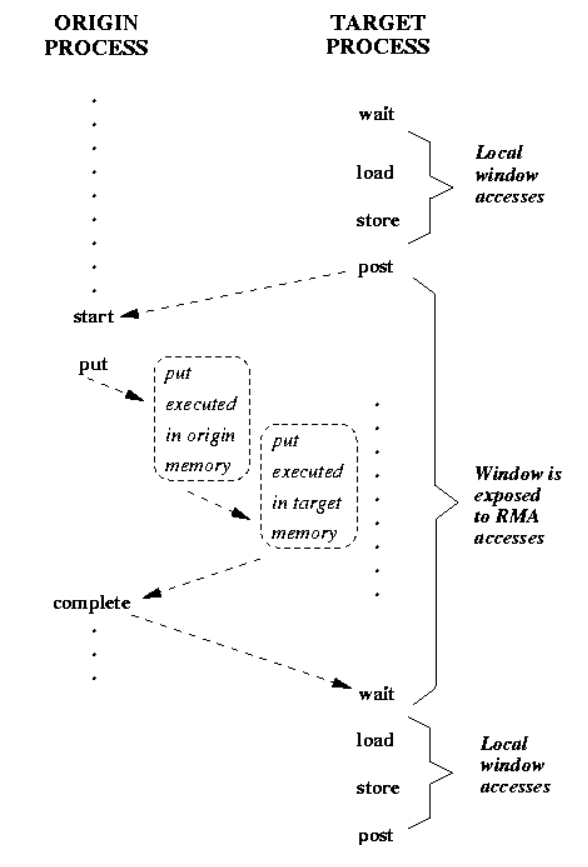
\includegraphics[width=0.65\textwidth]{Active_synchronization}
    \caption{Diagramatic representation of Active Synchronization}
    \label{fig:Active_synchronization}
\end{figure}

\subsubsection{Passive Synchronization}
\begin{itemize}
    \item Epochs for this synchronization are lock and unlock
    \item communication operations within epoch are all nonblocking
    \item the first origin process communicates the data to the second origin process, through the memory of the target process
    \item the target process is not explicity involved in the communication
\end{itemize}

\begin{figure}[h]
    \centering
    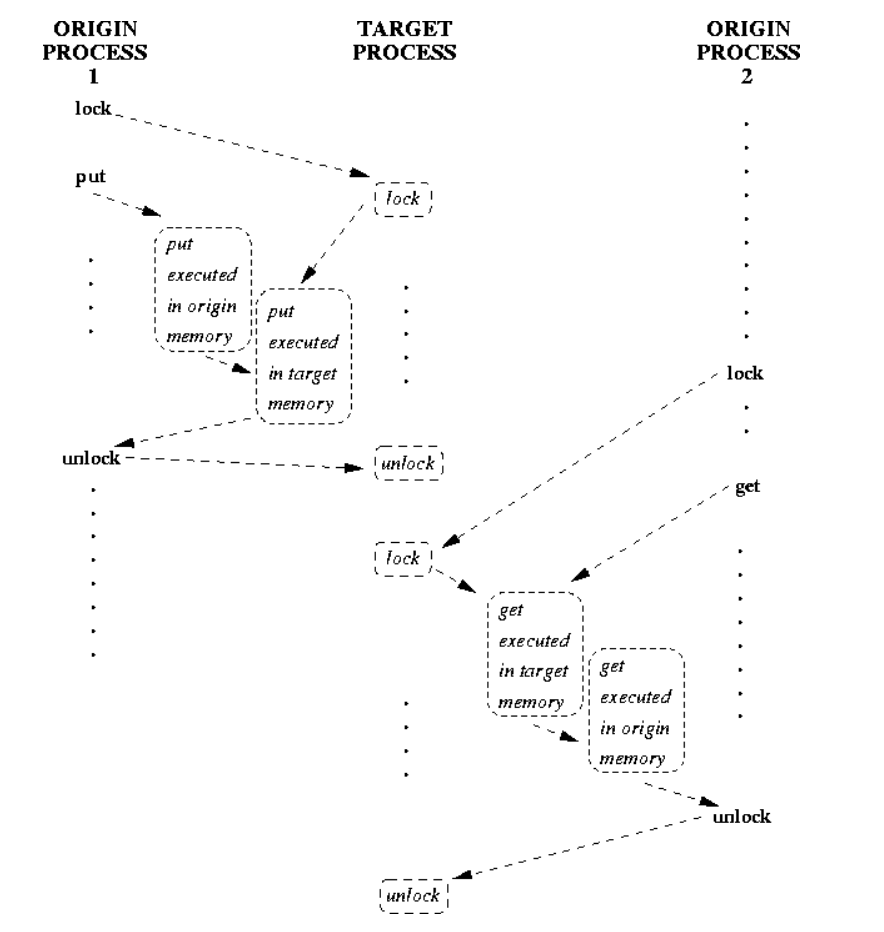
\includegraphics[width=0.65\textwidth]{Passive_synchronization}
    \caption{Diagramatic representation of Passive Synchronization}
    \label{fig:Passive_synchronization}
\end{figure}

\subsubsection{Difference between Active and Passive Synchronization}
The main difference between the Active and Passive Sychronization in MPI RMA/One-sided Communication is that {\bfseries{former the target is actively involed
in the communication}} by issuing commands for synchronization that are of blocking nature. However, in the latter, there is no issue of any such commands and
{\bfseries{the target is not explicity involved in the communications}}.

\section{Hybrid Programming: Combining Shared Memory and Distributed Memory Programming}
Nodes in distributed memory systems are shared memory nodes. The need for messaging library like MPI is only for cross-node communication. So, can performance 
be improved on the node?

{\bfseries{Option 1: MPI}}
\begin{itemize}
    \item advantageous since it uses one single model, portability
    \item disadvantages: no full use of sharing capabilities
    \item thus, there might be performance related issues
\end{itemize}
{\bfseries{Option 2}}: explores the idea of {\bfseries{Hybrid Programming}} which uses shared memory model within an MPI process. MPI + OpenMP is a typical option.

\subsection{Threading and MPI}
Base for any MPI program is a set of sequential programs typically one per base. Each calls \verb$MPI_Init$.

\subsubsection{What happens if one uses a threaded program as base?}
\begin{itemize}
    \item MPI 1.x was written without threads in mind
    \item It is for this reason that \verb$MPI_Init$ assumes single thread and MPI does not need to be thread safe
    \item Access from several threads can cause problems during execution
    \begin{itemize}
        \item shared data structures will require synchronization and need for some consistency model
        \item coordinate access to NIC
        \item call back coordination
    \end{itemize}
\end{itemize}

\subsection{MPI's Four Levels of Thread Safety}
New MPI Initialization routine:
\begin{verbatim}
    int MPI_Init_thread(    int *argc, char ***argv,
                            int required,
                            int* provided
                       );
\end{verbatim}
Application states needed level of thread support. MPI returns the one its supports.

\begin{itemize}
    \item \verb$MPI_THREAD_SINGLE$: only one thread exists in the application
    \item \verb$MPI_THREAD_FUNNELED$: multithreaded, but only the main thread makes the MPI calls
    \item \verb$MPI_THREAD_SERIALIZED$: multithreaded, but only one thread makes MPI calls at a time
    \item \verb$MPI_THREAD_MULTIPLE$: multithreaded and any thread can make API calls at any time
\end{itemize}

\subsubsection{Consequences of using \texttt{MPI\textunderscore THREAD\textunderscore MULTIPLE}}
\begin{itemize}
    \item Each call to MPI completes on its own and the effect is as if they would have been called sequentially in some order
    \begin{itemize}
        \item BLocking thread will only block the calling thread
    \end{itemize}

    \item User is responsible for making sure racing calls are avoided, for example: access to an already freed object
    \begin{itemize}
        \item Collective operations must be correctly ordered among the threads
    \end{itemize} 
\end{itemize}

\subsection{Threads-Levels when using OpenMP}
Similar to thread + MPI case, we use \verb$MPI_Init_thread$ to MPI with the right thread level.
\begin{itemize}
    \item \verb$MPI_THREAD_SINGLE$: there is no OpenMP multithreading in the program
    \item \verb$MPI_THREAD_FUNNELED$\\
          Must ensure that all the MPI calls are made by the master thread
          \begin{itemize}
              \item outside the parallel region
              \item during the master region
          \end{itemize}
          This happens to be the most common scenario
    \item \verb$MPI_THREAD_SERIALIZED$\\
          Must ensure that only one thread calls MPI at one time
          \begin{itemize}
              \item Critical or single regions
              \item through added synchronizations
          \end{itemize}
    \item \verb$MPI_THREAD_MULTIPLE$
    \begin{itemize}
        \item any thread can make an MPI call at any time
        \item also compatible with OpenMP tasking
    \end{itemize}
\end{itemize}

\subsection{Hybrid Programming: MPI + OpenMP}
OpenMP regions between MPI communications
\begin{itemize}
    \item Easy to understand
    \item Fits many programs
    \item Matches SPMD mode
    \item Required thread funneled only
\end{itemize}

The major disadvantage is {\bfseries{Amdahl's law in the non-OpenMP regions}}, i.e., complete parallelization of the program is not possible; at some points 
communication and synchronizations impacts the scalability of the parallelization.

{\bfseries{Best practice is follow Hierarchical Data Decomposition}}: \\
Need to split data structures(for MPI), then share data points(for OpenMP threads)

  


    




    







%==============================================CHAPTER 04===================================================
\chapter*{Conclusion}
And how it ends we shall decide later.





%==============================================REFERENCES===================================================
\newpage
\begin{thebibliography}{3}
  
\end{thebibliography}

\end{document}